% !TEX TS-program = pdflatexmk
\documentclass[pdflatex, sn-chicago]{sn-jnl}% Math and Physical Sciences Reference Style
\usepackage{anyfontsize}
\usepackage{lineno}
%%%% Standard Packages
\usepackage{mystyle}
\usepackage{tocloft}
\usepackage{etoc}
\setcounter{secnumdepth}{3}

%\usepackage[sectionbib]{chapterbib}
%\usepackage[backend=biber,style=authoryear]{biblatex}
%\usepackage{biblatex}
%\usepackage[natbib,style=authoryear, backend=biber]{biblatex}
%\addbibresource{biblio.bib}
\usepackage[resetlabels,labeled]{multibib}
\newcites{Main}{Bibliography}
\newcites{Meth}{Bibliography Methods}
\newcites{Supp}{Bibliography Supplementary Information}

\makeatletter
\renewcommand\@biblabel[1]{\textbullet} % Change the item label to a bullet, or customize as needed
\makeatother

\jyear{2021}%
%% as per the requirement new theorem styles can be included as shown below
\theoremstyle{thmstyleone}%
\newtheorem{theorem}{Theorem}%  meant for continuous numbers
%%\new-theorem{theorem}{Theorem}[section]% meant for sectionwise numbers
%% optional argument [theorem] produces theorem numbering sequence instead of independent numbers for Proposition
\newtheorem{proposition}[theorem]{Proposition}% 
%%\newtheorem{proposition}{Proposition}% to get separate numbers for theorem and proposition etc.

\theoremstyle{thmstyletwo}%
\theoremstyle{thmstylethree}%

\raggedbottom
%%\unnumbered% uncomment this for unnumbered level heads

\graphicspath{{./figures/}}

\begin{document}


\title[SatuTe]{\centering When the Past Fades: Detecting phylogenetic signal with SatuTe}

%%=============================================================%%
%% Prefix	-> \pfx{Dr}
%% GivenName	-> \fnm{Joergen W.}
%% Particle	-> \spfx{van der} -> surname prefix
%% FamilyName	-> \sur{Ploeg}
%% Suffix	-> \sfx{IV}
%% NatureName	-> \tanm{Poet Laureate} -> Title after name
%% Degrees	-> \dgr{MSc, PhD}
%% \author*[1,2]{\pfx{Dr} \fnm{Joergen W.} \spfx{van der} \sur{Ploeg} \sfx{IV} \tanm{Poet Laureate} 
%%                 \dgr{MSc, PhD}}\email{iauthor@gmail.com}
%%=============================================================%%

\author*[1]{\fnm{Cassius} \sur{Manuel}}\email{cassiusmanuelperez@gmail.com}
\equalcont{These authors contributed equally to this work.}
%cassius.perezdeloscoboshermtosa@meduniwien.ac.at
\author[1]{\fnm{Christiane} \sur{Elgert}}
\equalcont{These authors contributed equally to this work.}
\author[1,2]{\fnm{Enes} \sur{Sakalli}}
\equalcont{These authors contributed equally to this work.}
\author[1]{\fnm{Heiko A.} \sur{Schmidt}}
\author[4]{\fnm{Carme} \sur{Viñas}}

\author[1,3]{\fnm{Arndt} \spfx{von} \sur{Haeseler}} %\email{arndt.von.haeseler@univie.ac.at}
\affil[1]{\orgdiv{Center for Integrative Bioinformatics Vienna, Max Perutz Labs}, \orgname{University of Vienna, Medical University of Vienna}, \orgaddress{\street{Dr. Bohr Gasse 9}, \city{Vienna}, \postcode{A-1030}, \country{Austria}}}

\affil[2]{\orgdiv{Vienna BioCenter PhD Program}, \orgname{Doctoral School of the University of Vienna and Medical University of Vienna}, \orgaddress{\city{Vienna}, \postcode{A-1030}, \country{Austria}}}

\affil[3]{\orgdiv{Faculty of Computer Science}, \orgname{University of Vienna}, \orgaddress{\street{W\"ahringer Str. 29}, \city{Vienna}, \postcode{A-1090}, \country{Austria}}}

\affil[4]{\orgdiv{Faculty of Mathematics and Statistics}, \orgname{Polytechnic University of Catalonia}, \orgaddress{\city{Barcelona}, \country{Spain}}}
\linenumbers
\abstract{In phylogenetics, the phenomenon of saturation is well known, although its influence on tree reconstruction lacks a systematic and well founded method. Here we propose a new measure of the phylogenetic information shared between two subtrees connected by a branch in a phylogeny. This measure generalises the concept of saturation between two sequences to a theory of saturation between subtrees, whose implementation we provide as the versatile program SatuTe. We describe different usages of SatuTe, identifying which branches in a tree are phylogenetically informative and which alignment regions support a given branch. As an example, we discuss the Tree of Life reconstruction from ribosomal proteins and the 16S rRNA gene, with emphasis on the two-domain versus three-domain hypotheses. For the branch leading to Eukaryota, we show that most ribosomal proteins contain a strong phylogenetic signal, whereas some regions of the 16S rRNA gene have lost phylogenetic information. Thus, SatuTe opens new insights into phylogenetic inference and complements standard phylogenetic analysis.

}

\keywords{branch support, phylogenetic inference, phylogenetic signal, saturation, tree of life}

\maketitle

%%\pacs[JEL Classification]{D8, H51}

%%\pacs[MSC Classification]{35A01, 65L10, 65L12, 65L20, 65L70}

%\newpage
%\section*{}
%{\color{red} These are the format requirements of Nature methods:}
%
%    \noindent Abstract – up to 150 words, unreferenced. \\
%    Main text – 3,000 words (up to 5,000 words with editorial discretion), excluding abstract, Methods, references and figure legends.\\
%    Display items – up to 6 figures and/or tables. \\
%    Article should be divided as follows: \\
%    Introduction\\
%    Results\\
%    Discussion\\
%    Online Methods\\
%    References – as a guideline, we typically recommend up to 50.\\
%
%\medskip
%
%\noindent Proposed reviewers:
%
%Lars Jermiin - Lars.Jermiin@universityofgalway.ie
%
%Xuhua Xia - xxia@uOttawa.ca
%
%Maria Anisimovan - maria.anisimova@zhaw.ch
%
%David Duchene - david.duchene@sund.ku.dk.
%
%Simon Ho - simon.ho@sydney.edu.au
%
%Bernhard Misof - b.misof@leibniz-lib.de
%
%Karen Meusemann - k.meusemann@leibniz-lib.de

\newpage

\section*{Introduction}
Model-based phylogenetic inference has become common practice, largely due to the availability of phylogenetic software like PHYLIP \citepMain{felsenstein2005}, PhyML \citepMain{guindon2010}, RAxML \citepMain{Stamatakis2014} or IQ-Tree \citepMain{minh2020}. This practice involves inferring a phylogenetic tree from an multiple sequence alignment (MSA) and subsequently validating it using various statistical methods, such as the aLRT to evaluate the reliability of short branches \citepMain{Anisimova2006}. A popular method, the phylogenetic bootstrap, provides a support value for each branch in the tree, where a low bootstrap support value indicates that the branch has a poor reproducibility \citepMain{felsenstein1985confidence}. Conversely, branches with high bootstrap support values are considered as evidence of a real phylogenetic signal, justifying the separation between the two groups in the tree. Implicit to all these analyses is the assumption that the alignment contains sufficient phylogenetic information to conclude that the branch displays a historical relationship \citepMain{ho2004}.

\medskip
However, the antagonist to phylogenetic information is saturation, i.e., the occurrence of too many substitutions in an alignment to provide reliable information about true genetic distances \citepMain{philippe2011}. For two sequences, an alignment is considered saturated when it becomes impossible to determine whether the sequences are homologous or merely randomly related to each other \citepMain{jermiin2020, philippe1999, brown1982}. When two sequences are saturated, the evolutionary distance between them, measured in substitutions per site, is so extensive that their evolutionary relationship cannot be justified. Consequently, linking them with a branch to create the smallest possible tree lacks phylogenetic significance.

\medskip

For alignments with more than two sequences and a tree with many leaves, the question arises whether branches are subject to saturation and, more importantly, how to measure saturation.
If we detect saturation for a branch, then the phylogenetic signal for the two groups, separated by the branch, is so small that an evolutionary relationship among them is not justifiable.

\medskip 

Leaving aside the maximum-parsimony test  \citepMain{Archie1989} or ad hoc analyses \citepMain{liu2014, davalos2008}, tests for saturation consider entire alignments and their global phylogenetic signal \citepMain{duchene2021, xia2003index}. These methods do not consider the tree structure and thus cannot reveal saturation for individual branches in a phylogenetic tree.

\medskip

Here, we introduce SatuTe (\textit{Satu}ration \textit{Te}st), a new tool that fill a critical gap in the phylogenetic toolkit by detecting when sequence saturation hinders accurate inference of evolutionary relationships. For a phylogenetic tree and an alignment, SatuTe evaluates whether the alignment provides enough phylogenetic information to justify the branches in the tree. SatuTe embeds the analysis of saturation between two sequences into a general framework that handles multiple sequences and a tree. Thus, SatuTe opens a new avenue for studying the relationship between alignments and trees and helps to consolidate evolutionary conclusions.

\medskip

In the following, we present the theoretical foundations of SatuTe. We explain the test designed to reject the null hypothesis of saturation in favour of the alternative hypothesis of phylogenetic signal present. Alternatively, the p-value computed from our test statistic indicates the strength of evidence against the null hypothesis of saturation for a branch. We then       evaluated the performance of SatuTe on simulated alignments and investigate its applicability for typical phylogenetic questions. These questions focus on deciding whether a branch in the tree is supported by the phylogenetic signal of the alignment. Lastly, we use SatuTe to examine real data, analysing the phylogenetic signal of ribosomal protein and 16S rRNA alignments for the Tree of Life (ToL). We exemplarily analyse the branch connecting Eukaryota with the rest of the tree to shed new light on the ongoing debate between the two-domain hypothesis \citepMain{williams2D, Hug2016}  and the three-domain hypothesis \citepMain{woese, gribaldo2010}.

\section*{Results}
\subsection*{Foundations of SatuTe}\label{sec:SatuTe}
To keep the explanation simple, we present the 
theory and statistical method using DNA, though they are equally applicable to amino acid sequences.
For further details, we refer to Methods
 and Supplementary Information \ref{suppsec:maths}.

\medskip

Fig.\,\ref{fig:panel1}a displays an alignment of length $n$, where the columns of the alignment represent the $n$ site patterns $\partial$, while each of the $m$ rows represents a nucleotide sequence of the taxa comprising the leaves of a phylogenetic tree. We assume the GTR model, a reversible and stationary model of sequence evolution   with rate matrix $\bm{Q}$  and stationary nucleotide distribution $\bm{\pi}$ \citepMain{tavare1986}. The matrix $\diag (\bm{\pi})\bm{P}(t) = \diag (\bm{\pi})e^{\bm{Q}\cdot t}$ describes the probability of each nucleotide pair if $t$ substitutions per site (branch length) have occurred.

\medskip

For the model of sequence evolution and the phylogenetic tree, we ask if the branch $AB$ (Fig.\,\ref{fig:panel1}b) is supported by the phylogenetic signal provided by the alignment. To this end, we compute for site pattern $\partial$ the (partial) likelihood vectors $\va$ and $\vb$ at nodes A and B \citepMain{Felsenstein1981}, where $\partial A$ and $\partial B$ are the subpatterns of $\partial$
induced by branch $AB$. The probability of observing pattern $\partial$ of the alignment is
computed as

\begin{align} \label{eq:branch_likelihood_given_t} \Prob(\partial \mid t)  = \va^T \diag (\bm{\pi})  \bm{P}(t) \vb,
\end{align}

where $t$ is the branch length of $AB$. Moreover, the reversibility of the substitution model allows the spectral decomposition of matrix $\diag (\bm{\pi})\bm{P}(t)$ \citepMain{levin2017markov}, expressed as

%\begin{align} \label{eq:spectral_decomposition}
%   \bm{P}(t) = \bm{1}\cdot\bm{\pi}^T + \sum_{i=1}^3\bm{v_i}\cdot \bm{h_i}^T e^{\lambda_it},
%\end{align}

\begin{align} \label{eq:spectral_decomposition}
   \diag (\bm{\pi})\bm{P}(t) = \bm{\pi} \bm{\pi}^T + \sum_{i=1}^3\bm{h_i} \bm{h_i}^T e^{\lambda_it},
\end{align}
 
where  ${\lambda_0 = 0 > \lambda_1 \geq \lambda_2 \geq \lambda_3}$  are the eigenvalues of the rate matrix and $\bm{h_k}$  are the corresponding left eigenvectors ($i = 1,2,3$). 
%Note that the right eigenvalues form an orthonormal basis with respect to $\bm{\pi}$-inner product $\langle \bm{v},\bm{w}\rangle_{\bm{\pi}}= \bm{v}^T\cdot\diag(\bm{\pi})\cdot\bm{w}$ and $\bm{h}_k=\diag(\bm{\pi})\cdot\bm{v}_k$.

\medskip 

Substituting equation \eqref{eq:spectral_decomposition} into \eqref{eq:branch_likelihood_given_t}, we derive the central equation

\begin{align}\label{eq:branchlikelihod_new}
    \Prob(\partial \mid t)  = \Prob(\pred)\Prob(\pblue) +  \sum_{i =1}^3  \langle \va,\bm{h_i}\rangle \langle \vb, \bm{h_i}\rangle\, e^{\lambda_i t},
\end{align}

where $\langle\cdot,\cdot\rangle$ denotes the scalar product, and $\Prob(\pred) = \langle \va,\bm{\pi}\rangle$ , $\Prob(\pblue) = \langle \vb,\bm{\pi}\rangle$ are the probabilities for patterns $\pred, \pblue$ given subtrees $\mathbb{T}_A, \mathbb{T}_B$, respectively. Note that the product $\Prob(\pred)\Prob(\pblue)$ describes the probability of pattern $\partial$ if the subtrees are independent from each other.

\medskip

Rewriting Eq.\,\eqref{eq:branchlikelihod_new} in a more compact form, and assuming all eigenvalues are different, we obtain

\begin{align} \label{eq:centraleq} 
\frac{\Prob(\partial \mid t)}{\Prob(\pred)\Prob(\pblue)} =  1 + \sum_{i =1}^3 C^\partial_i  e^{\lambda_i t},
\end{align}

where  $C^\partial_i$ is given by
\begin{equation}
    C^\partial_i = \langle  \tfrac{\va}{\Prob(\pred)},\bm{h_i}\rangle \langle \tfrac{\vb}{\Prob(\pblue)}, \bm{h_i}\rangle.
\end{equation}

\medskip


Eq.\,\eqref{eq:centraleq} shows that with increasing branch length $t$, the ratio of the probability for pattern
$\Prob(\partial \mid t)$ for the tree and the product of the probabilities for the two subpatterns converges
exponentially quickly to one, since the non-zero eigenvalues $\lambda_i$ are negative.

\medskip 

Conversely, if $\mathbb{T}_A$ and $ \mathbb{T}_B$ are independent, then the sum in Eq.\,\eqref{eq:centraleq} must equal zero for all branch lengths $t$. While we cannot expect that this be true for an individual pattern $\partial$, we show that the expectation of any coefficient $C^\partial_i$, when summed over all patterns, equals zero if $\mathbb{T}_A$ and $\mathbb{T}_B$ are independent. We call $C^\partial_i$ the coherence coefficient (for the non-zero eigenvalue $\lambda_i$). Because the second largest eigenvalue $\lambda_1$ dominates the sum in Eq.\,\eqref{eq:centraleq}, we will restrict our analysis to the coherence coefficient $C^\partial_1$.

\medskip 

The expected coherence coefficient is estimated from the alignment and the tree as the average $\hat C_1 = (1/n)\sum_{s=1}^n C^{\partial_s}_1$ for the $n$ site patterns ${\partial_s}$. According to the central limit theorem, the average coherence coefficient is approximately normally distributed (Fig.\,\ref{fig:panel1}c) with expectation $0$ and standard error $\sigma_1/\sqrt{n}$, which can be estimated from the data (see Methods \ref{msec:estimates}). $\hat C_1$ can be z-transformed to obtain a normalised z-score $Z$. The null hypothesis that no phylogenetic signal exists to justify branch $AB$ is rejected if the z-score $Z$ is larger than the critical value $z_\alpha$ of a specified significance level $\alpha$ (Fig.\,\ref{fig:panel1}d).

\medskip

	\begin{figure}[H]
            \centering
            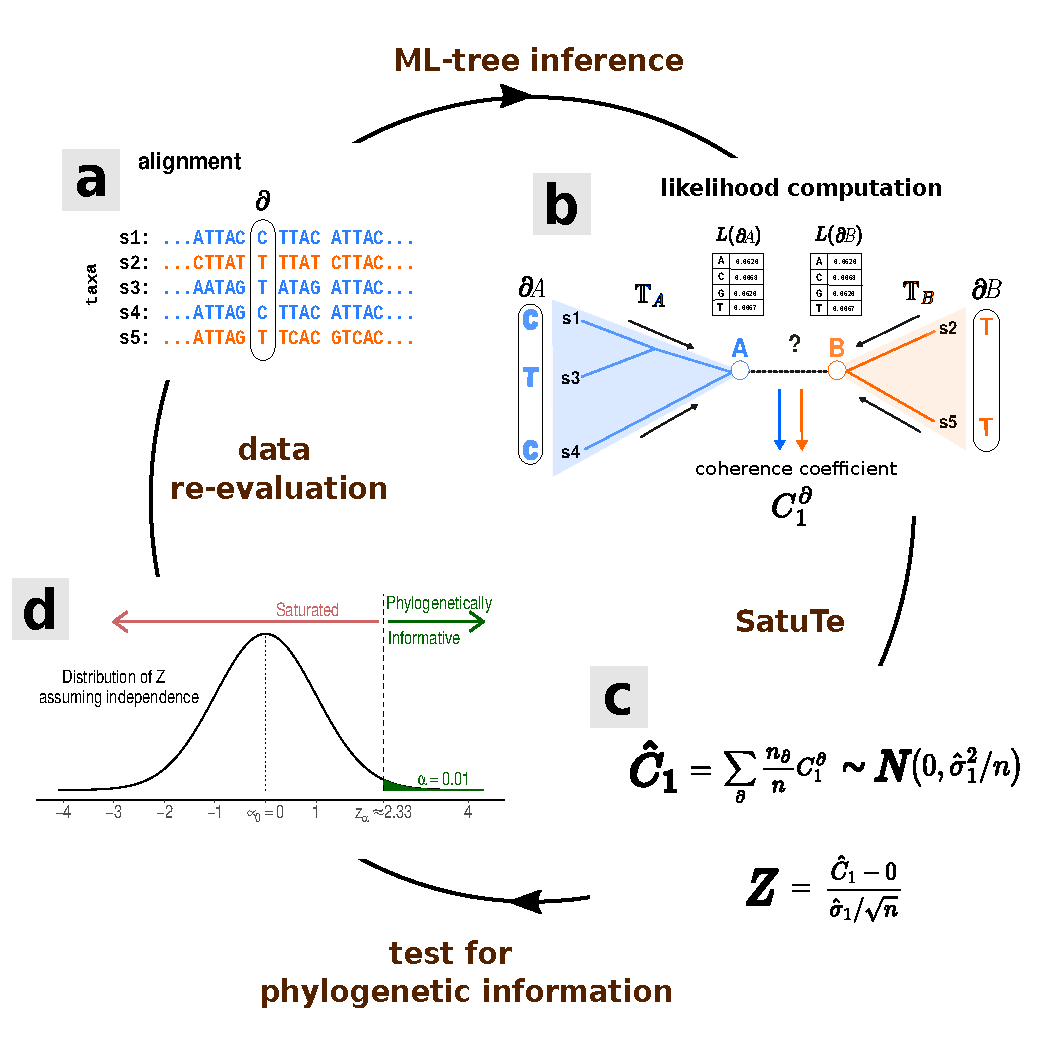
\includegraphics[width=\linewidth]{figure_1_2024_08_02.pdf}
		     \caption{
		   \textbf{SatuTe in a nutshell.} \textbf{(a)} Five-taxon DNA alignment where each column represents a pattern $\partial$. \textbf{(b)} The branch $AB$ splits the five-taxon tree into subtree $\mathbb{T}_A$ with sequences $S1,S3,S4$ and subtree $\mathbb{T}_B$ with sequences $S2, S5$. Additionally, branch $AB$ splits each pattern, such as $\partial = \text{CTTTC}$, into subpatterns ${\partial A=\text{CTC}}$ and ${\partial B=\text{TT}}$. These subpatterns are used to compute the likelihood vectors $\va$ and $\vb$, which determine the coherence coefficients. \textbf{(c)} The average coherence $\hat{C}_1$ is approximately normally distributed, with expectation zero and standard error
     $\hat{\sigma}_1/\sqrt{n}$, if the subtrees  $\mathbb{T}_A$ and  $\mathbb{T}_B$ are independent. The z-transform of the average coherence is then used to test for phylogenetic information. \textbf{(d)} The null hypothesis of independently evolving subtrees is rejected at the significance level $\alpha$ if $Z>z_\alpha$. Rejection implies phylogenetic signal. Thus, the subtrees share a common history and are connected by a branch.}
		     \label{fig:panel1}
        \end{figure}



\subsection*{SatuTe applied to simulated data}

We analysed the performance of SatuTe for a wide variety of parameter selections, including different numbers of taxa (five and sixteen), different alignment lengths ($100$, $1000$, $10000$), various branch types (internal, external) and different branch lengths for the branch $AB$ of interest (Fig.\,\ref{fig:simulation}). For each parameter
combination we simulated 1000 alignments along the specified tree assuming the Jukes-Cantor (JC) model \citepMain{Jukes1969}. For details of the simulation see Methods \ref{msec:simulations}. The parameter combinations reflect typical phylogenetic scenarios.

\medskip

In the \textbf{first scenario}, representing the statistically correct situation ({\color{truetree} pink}, Fig.\,\ref{fig:simulation}), the alignment is simulated along the true (simulation) tree with its true branch lengths. Subsequently, the phylogenetic signal of the simulated alignment was tested on the true tree
(including the true branch lengths) for the external edge (Fig.\,\ref{fig:simulation}a) and the internal edge (Fig.\,\ref{fig:simulation}b). Regardless of the specific parameters, the fraction of simulated alignments that are phylogenetically informative for branch AB decreases from 100\% to the significance level of 5\% as the
branch length increases. Thus, long branch lengths in the true evolutionary process resulted in lower rejection rates of the null hypothesis of subtree independence, leading to more instances where the subtrees lack a phylogenetic signal for $AB$. According to standard statistical theory, longer alignments preserve phylogenetic signal for longer branches, so the overall behaviour of the curves follows a typical power curve and serves as a basis for other scenarios that deviate from this gold-standard.

\medskip 


A realistic application similar to the first scenario is the following. After reconstructing a phylogenetic tree from a long (phylogenomic) alignment, one might want to identify which genes or regions are informative for the branches of the reconstructed tree. To achieve this, we analyse the reconstructed tree and test to which extent the genes or regions, which constitute only a fraction of the overall alignment, are phylogenetically informative.

\medskip 

Another application of SatuTe arised when we have a widely accepted tree and a new alignment for a gene family that has not yet been investigated. In this case, we would infer the branch lengths for the new alignment and check which branches in the accepted tree are supported by the new alignment. In other words, we determine where the new alignment is phylogenetically informative within the accepted tree topology. 

\medskip

This is what we consider in our \textbf{second scenario}  ({\color{truetreeML} purple}, Fig.\,\ref{fig:simulation}). Here, the true tree topology is known, but the branch lengths are maximum likelihood (ML) estimates based on the alignment. Fig.\,\ref{fig:simulation} shows that the purple curves are extremely close to the gold-standard (first scenario). For short sequences (100 sites), the test turns out to be too liberal, with an empirical rejection level of approximately 10\%, but we conclude that this is still tolerable.


\medskip


The \textbf{third scenario} ({\color{MLtree} blue}, Fig.\,\ref{fig:simulation}) involves reconstructing an ML-tree for an alignment and then determining where in the ML-tree the same alignment is phylogenetically informative. This scenario, where the data is used twice -- namely to infer the tree and then to investigate the phylogenetic signal of branches -- is known as circular analysis in statistics. Such double-dipping into the data undermines statistical inference and may lead to an inflation of the type I error \citepMain{button2019double}. This is actually what we observe in Fig.\,\ref{fig:simulation}, where for long branches 15\% of the alignments are tested as phylogenetically informative for the external branch (Fig.\,\ref{fig:simulation}a) and 50\% of alignments for the internal branch (Fig.\,\ref{fig:simulation}b), regardless of the sequence length. The high rejection rate is explained by the observation that for long branches AB most of the reconstructed trees disagree with the true tree. Most of the inferred ML-trees link subtrees $\mathbb{T}_A$ and $\mathbb{T}_B$  via their external branches (Supplementary Table \ref{supptab:placementAB}). Thus, if subtrees have $m_A$ and $m_B$ leaves, then the tree with the highest likelihood among $m_A\cdot m_B$ trees is selected, which happens to be phylogenetically informative.

\medskip

The \textbf{fourth scenario} shows that the Bonferroni adjusted significance level $\alpha_{adjust} = \alpha / (m_A m_B)$ provides power curves ({\color{MLtreeBonferroni} green}, Fig.\,\ref{fig:simulation}) that are close to the gold-standard. However, if the subtrees contain very similar sequences, then $\alpha_{adjust}$ may become too small (Supplementary Fig.\,\ref{suppfig:simulation_shortBranches}). Then it may help to reduce the number of leaves and to carry out additional simulations tailored for the specific question and data.

\medskip

Fig.\,\ref{fig:simulation} shows the results generated under the assumption that no model misspecification occurs. Since the computation of the coherence coefficient obviously depends on the selected model of sequence evolution, we evolved sequences under a GTR-model \citepMain{tavare1986} and then
inferred an ML-tree assuming either a JC or Kimura two parameter (K2P) \citepMain{kimura1980simple} model. In both cases we observe a too liberal test (Supplementary Fig.\, \ref{suppfig:simulation_misspec}), with too many alignments considered phylogenetically informative for the branch $AB$ compared to the gold-standard. However, when we replaced the JC or K2P model by the F81 model \citepMain{Felsenstein1981}, which incorporates the base composition of the alignment, SatuTe performed well and the power curves approach the gold-standard (Supplementary Fig.\, \ref{suppfig:simulation_misspec}).
Thus, the most critical aspect for the good performance of SatuTe is specifying the base composition, which is straightforward from the data. However, the estimation of the correct
substitution rate parameters in the rate matrix is less important.

\medskip 



%%% Fig 2 - simulation %%%
\begin{figure}[H]
    \centering
    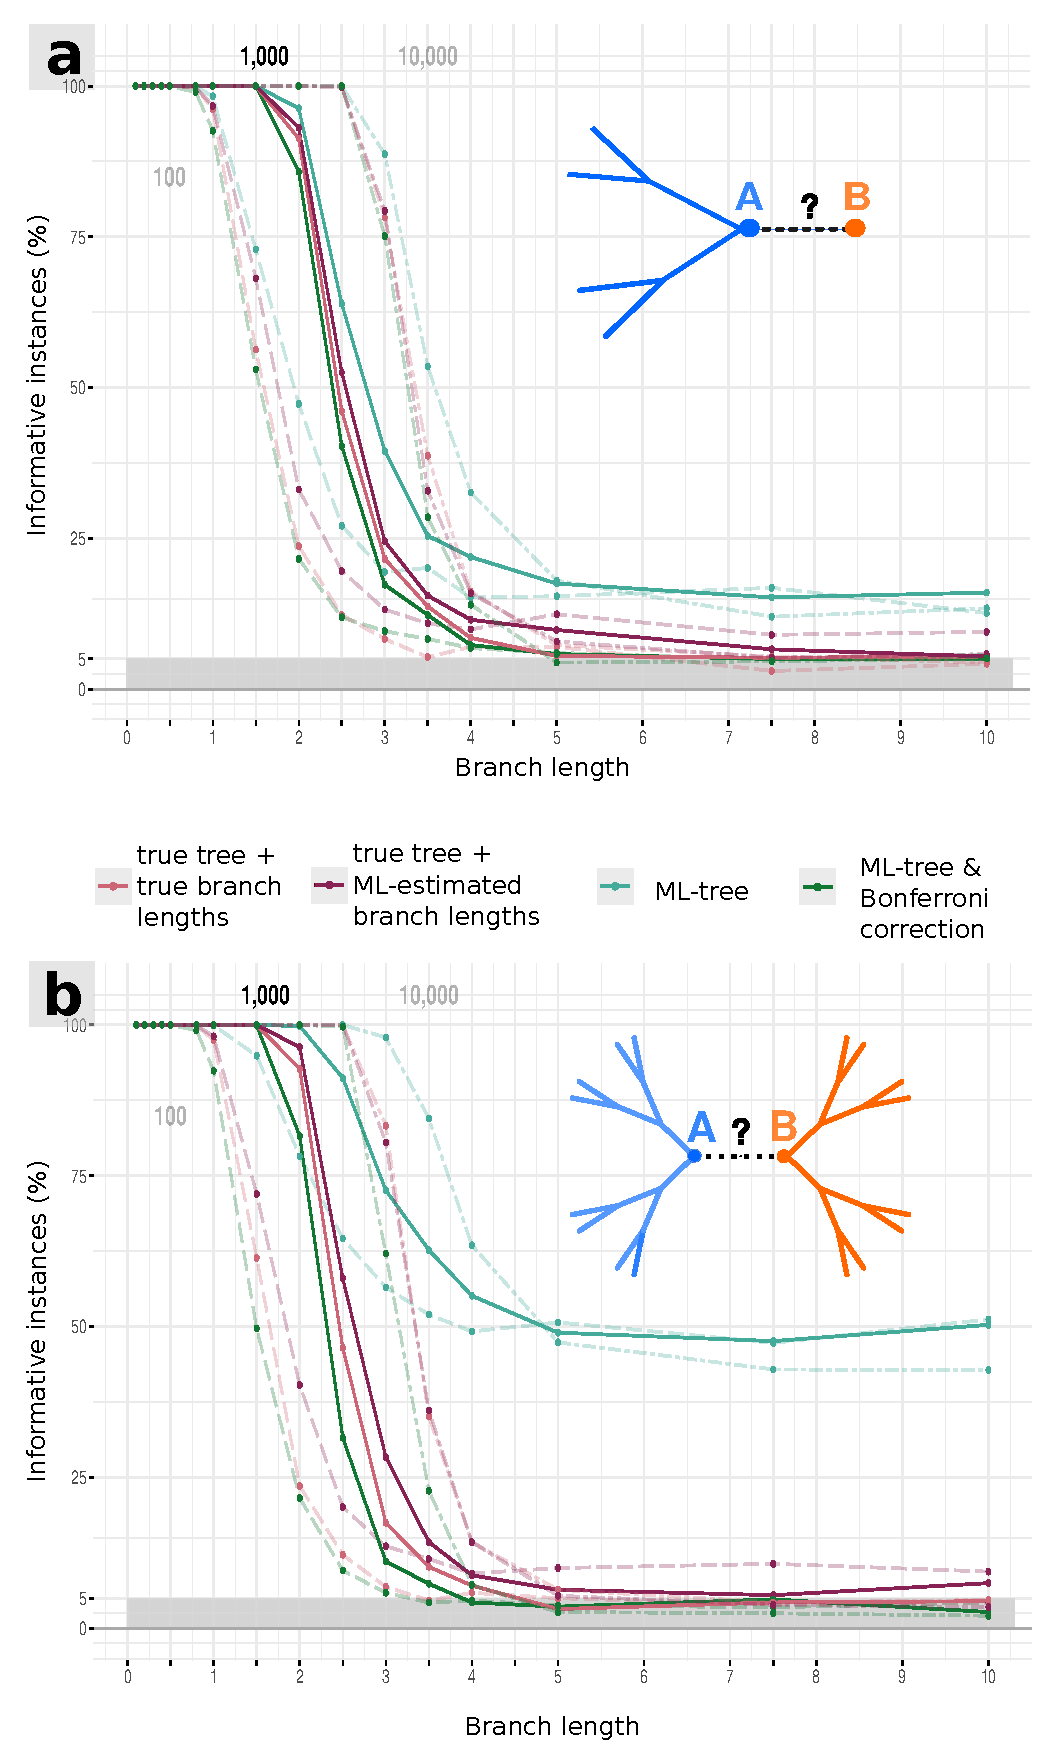
\includegraphics[scale=0.5]{figure_simulated_data_main.pdf}
     \caption{\textbf{Performance of SatuTe in simulations}. The plot shows the fraction of phylogenetically informative simulated alignments for branch $AB$ and various analysis scenarios: the true tree ({\color{truetree}pink}), the true tree topology with ML-estimated branch lengths ({\color{truetreeML} purple}), and the inferred ML-tree including branch lengths ({\color{MLtree} blue}). The {\color{MLtreeBonferroni} green} curves represent the percentage of informative instances after applying the Bonferroni correction to the light green instances. In \textbf{(a)}, an external branch of a five-taxon tree and in \textbf{(b)}, the central branch of a balanced 16-taxon tree is analysed. Dashed, solid, and alternating dashed lines represent the results for 100, 1000, and 10000 sites, respectively.}
     \label{fig:simulation}
\end{figure}


\subsection*{SatuTe investigates the Tree of Life}

We applied SatuTe to two alignments used to determine deep branching patterns in the ToL \citepMain{Hug2016}. The first alignment, comprising 16 ribosomal-subunit proteins, with a length of 2596 amino acid sites and 3083 taxa suggests the two-domain tree (2D ToL), in which the Eukaryota branch off within the Archaea (Fig.\,\ref{fig:EUK}a). The second alignment, consisting exclusively of the 16S rRNA gene with 1947 sites and 1871 taxa, supports the three-domain tree (3D ToL), in which Archaea, Bacteria and Eukaryota are each monophyletic (Fig.\,\ref{fig:EUK}d). Depending on the alignments the 2D ToL or 3D ToL is inferred (see \citetMain{Hug2016}). 

\medskip
To examine the phylogenetic information in both alignments, we  inferred the branch lengths for both trees, using the LG+G4 model for the protein alignment and the GTR+G4 model for the 16S rRNAs (Methods \ref{msec:ToL}). We have focused our analysis on the models considered by the authors, as exploring alternative models is beyond the scope of our study.

\medskip


Since the 2D ToL is based on an LG+G4 model and SatuTe is only applicable if all sites evolve at the same rate (Methods \ref{msec:hetero}), each alignment site was assigned to the rate category with highest posterior probability \citepMain{yang1994maximum}. For sites within each rate category, we determined the phylogenetic signal for each branch according to the fourth scenario (ML-tree \& Bonferroni correction). All 6163 branches were phylogenetically informative for each of the four rate categories. Fig.\,\ref{fig:EUK}b displays the z-scores for the Eukaryota branch and for comparison an external branch leading to yeast.

\medskip

For the 3D ToL we inferred the branch lengths with the GTR+G4 model and repeated the above analysis. From the 3739 branches, 107 branches were classified as saturated for sites from the highest rate category (rate 2.73). Among the saturated branches, there were 13 internal branches and one of them was the branch connecting Eukaryota with the rest of the tree
(Fig.\,\ref{fig:EUK}e). Thus, the fastest evolving sites in the 16S rRNA alignment do not provide support for the Eukaryota branch.

\medskip

Given these results, we decided to focus on the branch that separates the Eukaryota from the rest in both the 2D and 3D ToL. Using SatuTe, we conduct a sliding-window analysis with a window size of 36 sites for both alignments (Methods \ref{msec:ToL}) to identify which regions of each alignment are phylogenetically informative for the Eukaryota branch. As the window length is small in relation to the total alignment, the analysis per window is similar to the first scenario of the simulations. Figs.\,\ref{fig:EUK}c and \ref{fig:EUK}f show the z-scores along the alignment. The ribosomal proteins show a clear phylogenetic signal for the entire alignment. The signal seems to be strong  independently of the proteins. Only a few short regions exist where the phylogenetic signal has been lost (that is, z-score falls below the critical value $z_{\alpha}$). These regions are often found at the junction of two concatenated protein alignments. For the 3D ToL determined from the 16S rRNA alignment, we find many and sometimes very long alignment regions that are not phylogenetically informative (Fig.\,\ref{fig:EUK}f). Saturated regions are mostly found in the so-called hypervariable regions V1-V9 \citepMain{baker2004}. On the other hand, from the conserved regions C1-C9 in bacteria \citepMain{yang2016}, regions C1 and C4-C9 show phylogenetic signal, whereas C2 and C3 are almost saturated (for the Eukaryota branch). The conspicuously long phylogenetically uninformative regions 240-301 (z-score $< 1 \cdot 10^{-16}$)
and 789-956 (z-score $< 1 \cdot 10^{-14}$) of the alignment have a low z-score because they are gappy and therefore provide little information about the substitution model.

\medskip 

The sliding-window analysis of the 16S rRNA revealed that 43.0\% of the 1912 windows show no phylogenetic signal for the Eukaryota branch. In the protein alignments we only find 5.4\% saturated windows. Even if the protein alignments have conserved significantly more phylogenetic information from early evolution, we currently cannot decide whether the
3D ToL is an artefact due to many saturated regions in the alignment. SatuTe does test for saturation but does not determine which tree is correct. In any case, some regions of the 16S rRNA provide little phylogenetic information for the placement of the Eukaryota branch in the 3D ToL, as is evident from the z-scores (Fig.\,\ref{fig:EUK}f).

\medskip 

Finally, we note that the z-score can tell us "how much" phylogenetic information is present for branches in different trees that induce the same partition of taxa. In this specific case, we calculated for the ribosomal proteins the z-scores for the Eukaryota branch in the 2D ToL and the 3D ToL (Fig.\,\ref{fig:z-score_differences}a). The tree in Fig.\,\ref{fig:z-score_differences}a shows the possible placements of the Eukaryota branch. To get the 3D ToL for the protein alignment, we pruned the Eukaryota subtree from the 2D-tree and regrafted it on the branch connecting  Bacteria and Archaea. Then, following the second scenario, the ML-branch lengths were estimated for the rearranged tree and a LG+G4 substitution model. Supplementary Table \ref{supptab:protein_2D_3D} shows that the z-scores are significant for each protein, irrespective of 2D or 3D ToL. This suggests the presence of a phylogenetic signal that is independent of the trees. However, the 2D ToL z-scores are slightly larger except for proteins L15, L22 and S10 (Fig.\,\ref{fig:z-score_differences}b) and almost identical for L2. 
%
%
%
We analysed the 16S rRNA alignment in a similar way. Therefore, we performed the subtree and regrafting procedure on the 3D tree (Fig.\,\ref{fig:EUK}d) to obtain the 2D ToL (Fig.\,\ref{fig:z-score_differences}c). The 16S rRNA alignment was divided into 9 regions and for each region the z-score of the 2D ToL, 3D ToL and the region specific z-score differences were determined (Supplementary Table \ref{supptab:rRNA_2D_3D}). For six of the nine regions, the z-score difference is negative, i.e. these regions have a higher score in the 3D ToL (Fig.\,\ref{fig:z-score_differences}d).

\medskip

Interestingly, the empirical distributions of the z-score differences for both alignments show no significant difference (Kolmogorov-Smirnov test: p-value=0.072). In summary, for the 16S rRNA alignment it is not clear which tree to prefer. However, the analysis yields valuable insights into the phylogenetic information that individual alignments (different protein or different regions) provide for branches in a phylogenetic tree.

\begin{figure}[ht]
\centering
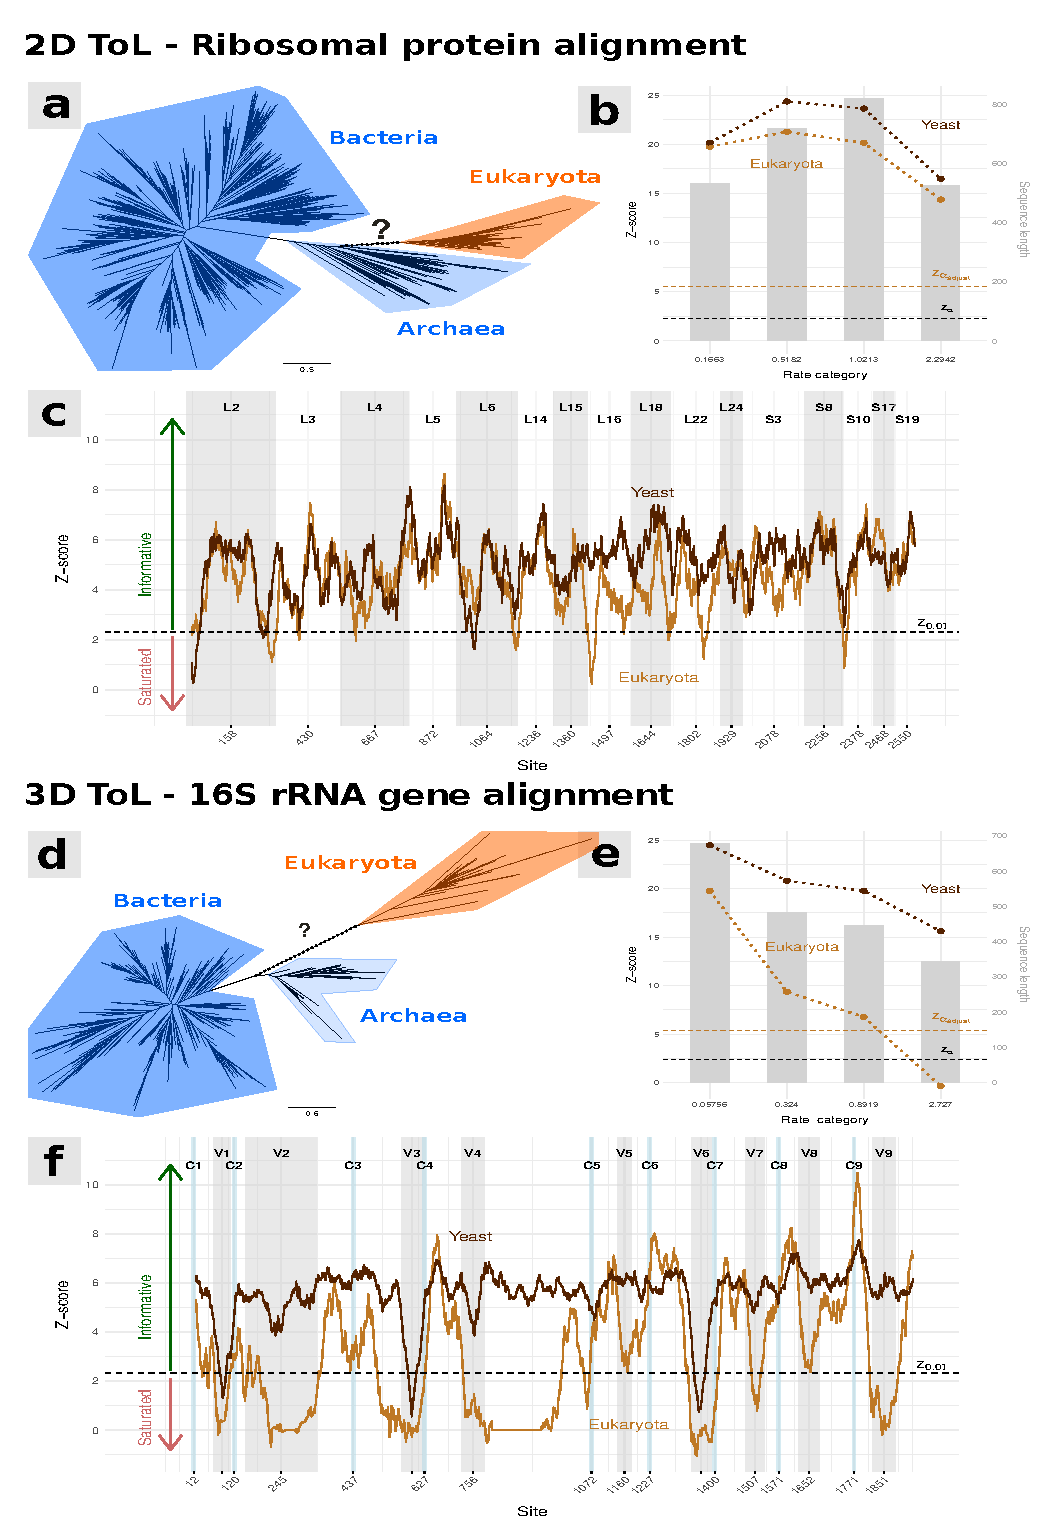
\includegraphics[width=\linewidth]{figure_sliding_window_2024_08_28.pdf}
	\caption{\textbf{Per rate category and sliding-window analysis of selected branches:} The branches leading to Eukaryota and yeast were analysed. \textbf{(a)}, 2D tree with $3083$ taxa obtained from the ribosomal protein alignment and \textbf{(d)}, 3D tree with 1871 taxa obtained from the 16S rRNA gene alignment. \textbf{(b)}, \textbf{(e)} The per rate category z-scores are marked as dotted lines, and the estimated number of sites per category is represented by grey bars. For the Eukaryota branch the Bonferroni adjusted critical value is shown.
 \textbf{(c)}, \textbf{(f)} The progression of the z-score was calculated as a moving average for a sliding window with 36 sites.
 }  \label{fig:EUK} 
\end{figure}


\begin{figure}[ht]
    \centering
    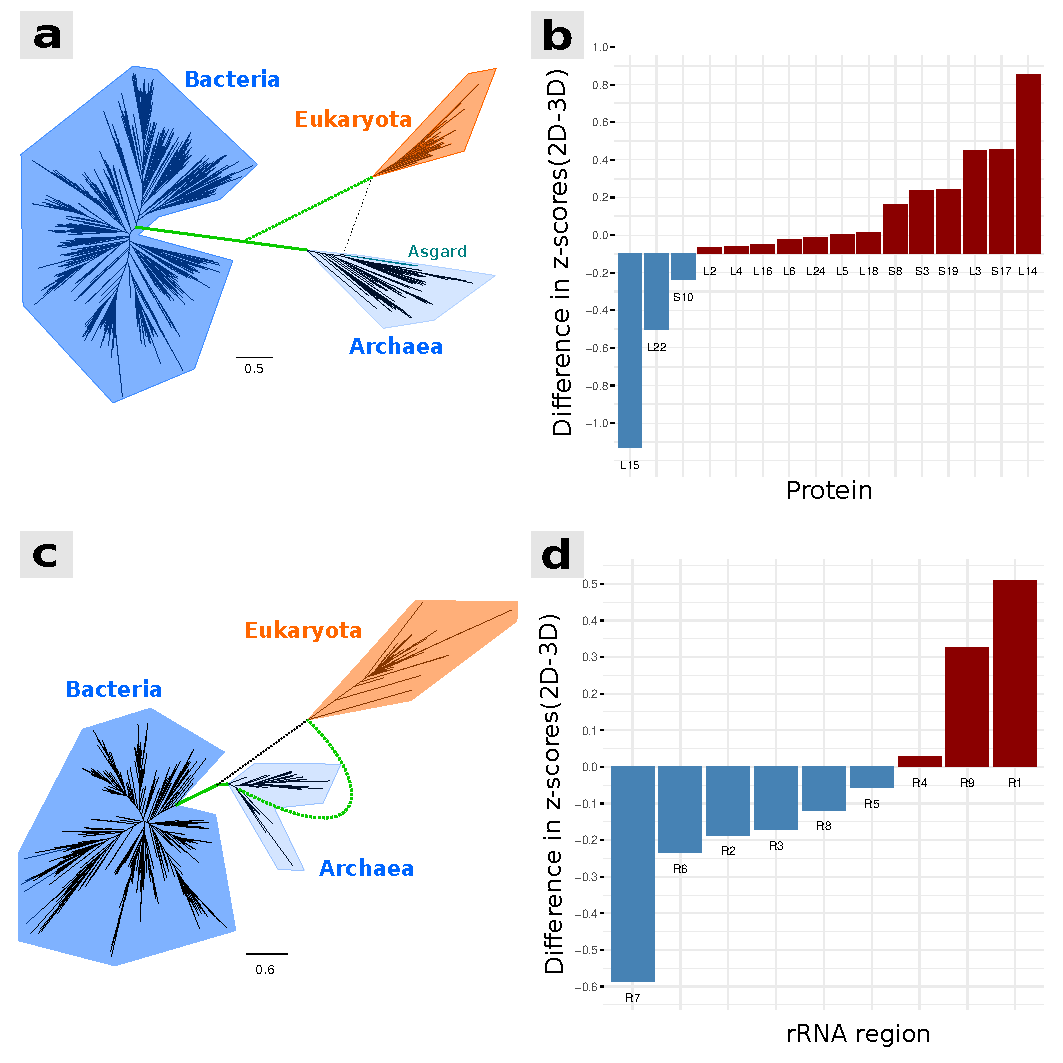
\includegraphics[width=\linewidth]{figure_zscore_differences_2024_08_06.pdf}
    \caption{\textbf{Differences between z-scores for the two placements of Eukaryota.} The topology rearrangement of \textbf{(a)}  the protein-based 2D tree (Fig. \ref{fig:EUK}a) into a 3D-tree  and \textbf{(c)} the 16S rRNA-based 3D tree (Fig. \ref{fig:EUK}d) into a 2D-tree by replacing the black dashed branch with the green dashed branch. For each \textbf{(b)} ribosomal protein and \textbf{(d)} rRNA region, the z-score differences of the branch leading to Eukaryota between the 2D-tree  and the 3D-tree are presented in ascending order.
    } \label{fig:z-score_differences} 
\end{figure}
\bigskip

\section*{Discussion}


SatuTe is a new method to quickly and efficiently compute the phylogenetic signal for every branch in a phylogenetic tree and a multiple sequence alignment. The practical applications of SatuTe are numerous and we have shown only some typical scenarios with simulated alignments and other applications based on alignments used in the discussion about the structure of the ToL \citepMain{williams2D,cunha3D}. The simulations show that SatuTe has all the properties of a good test and is also relatively robust when the ideal statistical conditions are not met. Our experiments (simulations, ToL) reflect typical applications of SatuTe. Many other analyses are conceivable.
To this end, we developed the SatuTe program package, which can be seamlessly integrated into a phylogenetic pipeline with IQ-Tree2, as a good and flexible starting point for more in-depth studies. SatuTe generates a comprehensive output for each alignment site, enabling further in-depth analysis, such as user-specific investigations of subregions, structural elements or other parts of an alignment. Additionally, the z-scores enable the comparison between branches in a tree or even between trees. We have presented the principle of this analysis in the ToL example. A more detailed analysis, which obviously depends on the data and the specific scientific questions, is beyond the scope of the paper. However, SatuTe offers the bioinformatic tools and the essential statistics to estavlish the groundwork for such an in-depth analysis.  

\medskip

That is why we did not resolve the discussion about the true phylogenetic relationship of Archaea, Bacteria and Eukaryota. Our analysis clearly highlighted strengths and weaknesses of the alignments that led to the conflicting hypotheses about the ToL. SatuTe helps to come to a more objective decision which alignments to include or exclude in a phylogenetic study. 

\medskip

SatuTe may be seen as a complementary tool to bootstrap methods  \citepMain{lemoine2018,hoang2017,Stamatakis2008,felsenstein1985confidence}, which measure how strongly an alignment supports a split between two groups. In the classic bootstrap interpretation, a high bootstrap value is taken as a consistency value for the branch in the tree. SatuTe helps to determine whether the two groups are related, i.e. that a branch indicates a common evolutionary history or if the high bootstrap value simply reflects the dissimilarity between the groups (Supplementary Table \ref{supptab:bootstrap}).

\medskip

The basic theory behind SatuTe gives additional information about the fading of the phylogenetic signal as the number of substitutions grows. As is well known \citepMain{levin2017markov,elchanan2003} the second largest eigenvalue describes the speed of the substitution model towards the stationary distribution. For the ToL discussion the second
largest eigenvalue of the LG+G4 model equals -0.27 and -0.83 for the GTR+G4 model. Therefore, the accelerated loss of phylogenetic signal along a branch under the GTR model, occurring three times faster offers at least a partial explanation for the preference of proteins in inferring deep phylogenies. This may also lead to a more systematic understanding for the usefulness of substitution models for inferring deep phylogenies \citepMain[see][]{kapli2023}.

\medskip 

Moreover, the computation of the coherence coefficient can be formally generalised for non-stationary and non-reversible substitution models using the $\bm{\pi}$-scalar product \citepMain{levin2017markov} between the likelihood vectors \citepMain{manuel2022}. However, dropping those assumptions leads to root identifiability issues. This implies that the test for saturation does not depend only on the parent node of the two subtrees, but also on the placement of the root. This complication leads to a slightly more technical test, that will be implemented in future versions of SatuTe.

\medskip

In summary, SatuTe enables completely new possibilities for phylogenetic analysis. We were only able to demonstrate some typical applications that look promising. Our software package, SatuTe, allows even the uninitiated to quickly carry out the presented applications. Additionally, SatuTe provides a detailed output for each alignment position, which can then be analysed for further questions.


\bigskip

%\section*{Online content}
%{\color{blue}Any methods, additional references, Nature Portfolio reporting summaries, source data, extended data, supplementary information, acknowledgements, peer review information; details of author contributions and competing interests; and statements of data and code availability are available at  }


\backmatter
 
% To change the title from References to Bibliography:


%\renewcommand\refname{Bibliography}
\bibliographystyleMain{apalike}
\bibliographyMain{biblio.bib} 


%\begin{refsection}
%\nocite{manuel2022}
%\printbibliography
%\end{refsection}
%\begin{refsection}
\addtocontents{toc}{\protect\setcounter{tocdepth}{0}}
\setlength{\parindent}{0pt}
\specialsection{Methods}

\subsection{Estimates for SatuTe}\label{msec:estimates}

The formal proofs of this section are to be found in Supplementary Information \ref{suppsec:maths}. Here we consider first the JC model, which has only two eigenvalues, with the second largest — of particular interest — having a multiplicity of three, i.e. $\lambda_1=\lambda_2 =\lambda_3$. This case is analogous to the general case where the second largest eigenvalue has any multiplicity greater than one. For the JC model, the central equation Eq.\,\eqref{eq:centraleq} can be written as 

\begin{equation} \label{eq:likelihood_branch_at_site_t33} \frac{\Prob(\partial \mid t)}{\Prob(\pred)\Prob(\pblue)} =  1 + \Big(\sum_{k=1}^3 \langle \tfrac{\va}{\Prob(\pred)},\bm{h_k}\rangle \langle \tfrac{\vb}{\Prob(\pblue)}, \bm{h_k}\rangle \Big) e^{\lambda_1 t}.
\end{equation}
Then the coherence coefficient corresponding to the second largest eigenvalue equals
\begin{align*}
    C_1^\partial =  \sum_{k=1}^3 \langle \tfrac{\va}{\Prob(\pred)},\bm{h_k}\rangle \langle \tfrac{\vb}{\Prob(\pblue)}, \bm{h_k}\rangle = \sum_{k=1}^3 C_{1,k}^\partial,
\end{align*} where $\bm{h_k}$ are the left eigenvectors and  $C_{1,k}^\partial$ are the coherence coefficients corresponding to the eigenvectors. 

\medskip

Given an alignment with $n$ sites, we compute the empirical mean as an estimator for the random variable $C_1^\partial$,

\begin{align} \label{eq:estimator_explicit}
    \hat C_1 := \frac{1}{n}\sum_{s=1}^n C_{1}^{\partial_s} = \frac{1}{n}\sum_{s=1}^n C_{1,1}^{\partial_s}+C_{1,2}^{\partial_s}+C_{1,3}^{\partial_s}
\end{align}

From the theory (Supplementary Information C), we know that the expected value for the coherence coefficients $C_{1,k}^\partial$ is zero, under the null hypothesis of subtree independence. Due to the linearity of the expectation, this also holds for $C_1^\partial$, i.e. $\mathbb{E}[C_1^\partial] = 0$.

\medskip

It is well known that for a sum of random variables, the variance is equal to the sum of all pairwise covariances: 

\begin{align*}
    \mathrm{Var}[C^\partial_1] = \mathrm{Var}\Big[\sum_{k=1}^3 C_{1,k}^\partial\Big] = \sum_{i,j=1}^3 \mathrm{Cov}\big(C_{1,i}^\partial,\,C_{1,j}^\partial\big)
\end{align*}

Note that $\mathrm{Cov}\big(C_{1,i}^\partial,\,C_{1,i}^\partial\big) = \mathrm{Var}[C^\partial_{1,i}]$.  Furthermore,  the covariance of two random variables can be calculated as the expected value of their product minus the product of their expected values, i.e., for our case:

\begin{align*}
    \mathrm{Cov}\big(C_{1,i}^\partial,\,C_{1,j}^\partial\big) = \mathbb{E}\big[C_{1,i}^\partial\cdot C_{1,j}^\partial\big] - \underbrace{\mathbb{E}\big[C_{1,i}^\partial\big]}_{=0}\cdot \underbrace{\mathbb{E}\big[C_{1,j}^\partial\big]}_{=0}.
\end{align*}

Since we already know that the expected values of $C_{1,k}^\partial$ is zero, the last term in the above equation is zero. %Let us now look at the expected value of the product and plug in their definition. Then, by simply rearranging the factors and subsequently using subtree independence, we can obtain the following:
To compute the expectation of the product of two coherence coefficients, we note under the null hypothesis of subtree independence that:
%By leveraging subtree independence and recognizing the multiplicative nature of expectations under independence, we get:

\begin{align*}
\mathbb{E}\big[C_{1,i}^\partial\cdot C_{1,j}^\partial\big] &= \mathbb{E}\Big[\underbrace{\langle \tfrac{\va}{\Prob(\pred)},\bm{h_i}\rangle \langle \tfrac{\vb}{\Prob(\pblue)}, \bm{h_i}\rangle}_{=C_{1,i}^\partial} \cdot \underbrace{\langle \tfrac{\va}{\Prob(\pred)},\bm{h_j}\rangle \langle \tfrac{\vb}{\Prob(\pblue)}, \bm{h_j}\rangle}_{= C_{1,j}^\partial} \Big]\\
&=\mathbb{E}\Big[\langle \tfrac{\va}{\Prob(\pred)},\bm{h_i}\rangle  \langle \tfrac{\va}{\Prob(\pred)},\bm{h_j}\rangle \cdot \langle \tfrac{\vb}{\Prob(\pblue)}, \bm{h_i}\rangle\langle \tfrac{\vb}{\Prob(\pblue)}, \bm{h_j}\rangle \Big]\\
&=\underbrace{\mathbb{E}\Big[\langle \tfrac{\va}{\Prob(\pred)},\bm{h_i}\rangle  \langle \tfrac{\va}{\Prob(\pred)},\bm{h_j}\rangle \Big]}_{=\sigma^2_{A,i,j}}\cdot \underbrace{\mathbb{E}\Big[ \langle \tfrac{\vb}{\Prob(\pblue)}, \bm{h_i}\rangle\langle \tfrac{\vb}{\Prob(\pblue)}, \bm{h_j}\rangle \Big]}_{=\sigma^2_{B,i,j}},
\end{align*}
because the expected value is multiplicative under independence. Note that each expectation $\sigma^2_{A,i,j}$ and $\sigma^2_{B,i,j}$ is associated with one of the subtrees. 
If a subtree, e.g. $\mathbb{T}_A$, consists of a single leaf, then $\sigma^2_{A,i,j}=\delta_{ij}$, where $\delta_{ij}$ is the Kronecker delta, defined as $\delta_{ij} = 1$ if $i=j$ and $0$ if $i \neq j$. Otherwise, the expectation $\sigma^2_{A,i,j}$ is estimated from the alignment using the empirical mean. 

\medskip

Therefore, the variance of the coherence coefficient  $\mathrm{Var}[C^\partial_1]$ can be estimated from the alignment as
\begin{align}\label{variance_estimate}
\hat\sigma_1^2= \sum_{i,j=1}^3 \hat\sigma^2_{A,i,j}\cdot \hat\sigma^2_{B,i,j}, 
\end{align}
where

\begin{align*}
    \hat{\sigma}^2_{A,i,j} :=
    \begin{cases}
    \frac{1}{n}\sum_{s=1}^n \,\langle \tfrac{\mathbf{L}(\partial_sA)}{\Prob(\partial_sA)},\bm{h_i}\rangle\langle \tfrac{\mathbf{L}(\partial_sA)}{\Prob(\partial_sA)},\bm{h_j}\rangle,  & \text{for internal node A},\\
    \delta_{ij},&  \text{for leaf A},
    \end{cases}
\end{align*}
and $\hat{\sigma}^2_{B,i,j}$ is constructed analogously.

\medskip

In contrast to the JC model, the second largest eigenvalue of a typical GTR model has multiplicity one, which leads to a variance of the coherence coefficient $C_1^\partial$ of

\begin{align*} 
\mathrm{Var}[C^\partial_1] = \mathbb{E}[(C^\partial_1)^2] - 0^2 = \mathbb{E}\Big[ \langle \frac{\va}{\Prob(\pred)}, \bm{h_1}\rangle^2 \Big] \cdot \mathbb{E} \Big[ \langle \frac{\vb}{\Prob(\pblue)},\bm{h_1}\rangle^2 \Big]
\end{align*}

and a simpler estimator of the form
\begin{align} \label{varciance_estimate_multi1}
  \hat \sigma_1^2 = \hat\sigma^2_{A,1} \cdot \hat\sigma^2_{B,1}
\end{align}

\begin{align*}
    \hat{\sigma}^2_{A,1} :=
    \begin{cases}
    \frac{1}{n}\sum_{s=1}^n \,\langle \tfrac{\mathbf{L}(\partial_sA)}{\Prob(\partial_sA)},\bm{h_1}\rangle^2,  & \text{for internal node A},\\
    \delta_{ij},&  \text{for leaf A},
    \end{cases}
\end{align*}
and $\hat{\sigma}^2_{B,1}$ is constructed analogously.

\medskip 

Note that we have presented the estimators for the coherence coefficients with respect to the second largest eigenvalue $\lambda_1$. However, this can also be done for any other eigenvalue in the same way.

\bigskip

\subsection{The test for phylogenetic information}\label{msec:test}

For a large alignment and independently evolving sites, our estimates are sufficiently accurate. According to the central limit theorem, $\hat C_1$ is normally distributed with an expectation of  0 and  a variance of $\hat\sigma^2_1/n$. As in a typical one-sided z-test, we reject the null hypothesis of independently evolving subalignments at a given significance level $\alpha$ if the z-score $Z$ satisfies
\begin{equation} \label{eq:th_zscore}
Z := \frac{\hat C_1 - 0}{\hat{\sigma}_1/\sqrt{n}} > z_\alpha,
\end{equation}
where $z_\alpha$ is the $\alpha$-quantile of the standard normal distribution, satisfying $\Pr(Z > z_\alpha) = \alpha$.

\medskip

If we reject independence, we conclude that the branch is phylogenetically informative, indicating that the subalignments share enough phylogenetic information to justify the connection in the tree. Otherwise, the branch is considered saturated. 


\medskip

The preceding theoretical results were derived under the assumption that the alignment and the placement of branch $AB$ are independent of each other. However, in practice, the placement is usually inferred from the alignment itself. To roughly correct for the double-dipping, we can apply the multiple-test Bonferroni correction to the number of pairs of leaves used to place branch $AB$. Specifically, we adjust the significance level $\alpha$ to \begin{equation} \label{eq:corrected_significance}
\alpha_{adjust} =  \frac{\alpha}{m_A\cdot m_B}, 
\end{equation}
where $m_A$ and $m_B$ are the number of leaves in subtree  $\mathbb{T}_A$ and $\mathbb{T}_B$, respectively. 

\bigskip

\subsection{SatuTe with rate heterogeneity model}\label{msec:hetero}

If an evolutionary model with rate heterogeneity is used, each site is assigned to the rate category with highest posterior probability \citepMeth{yang1994maximum}. Then, for each category $c$, SatuTe employs the test for phylogenetic information as described in Methods \ref{msec:test} on the rescaled phylogenetic tree  and the subalignment of the considered category. In this process, SatuTe determines for each category $c$  the variance estimator $\hat\sigma^2_{1,c}$ according to Eq.\, \eqref{variance_estimate}.

\medskip 

However, to  test  regions of  an alignment, such as in a sliding-window analysis, we need to calculate an global variance estimator because the regions consist of  sites belonging  to different categories. For simplicity, consider four rate categories. Each category $c$ has $n_c$ sites assigned. If the alignment has $n$ sites, the global variance can be calculated as weighted average of the category variance estimates:
\begin{align}\label{eq:global_variance}
\hat\sigma_1^2 := \sum_{ i= 1}^4\frac{n_{c_i}}{n}\cdot \hat\sigma^2_{1,{c_i}}.
\end{align}

For an alignment window of size $w$, we perform the test according to \ref{msec:test}, using the average of all coherence coefficients  over the $w$ sites within the window for the estimate $\hat C_1$ and  the standard error $\hat\sigma_1/\sqrt{w}$, where $\hat\sigma_1^2$ is obtained from Eq.\eqref{eq:global_variance}. 
We recommend a minimal sliding-window size of 30 sites, to ensure that the Central Limit Theorem is applicable.

\bigskip

\subsection{SatuTe in simulations}\label{msec:simulations}

We consider different simulation trees (see Table\,\ref{tab:Fig2}) with a branch $AB$ connecting the subtrees $\mathbb{T}_A$ and $\mathbb{T}_B$. The branch length of $AB$ was varied among $\{0.1, 0.2, 0.3, 0.4, 0.5, 0.8, 1.0, 1.5, 2.0, 2.5, 3.0, 3.5, 4.0, 5.0, 7.5, 10.0\}$. For each parameter combination, we simulated  $1000$ DNA alignments with sequence length ${n = 100, 1000, 10000}$ sites using Seq-Gen \citepMeth[v1.3.4;][]{Rambaut1997} under the JC model. Each alignment was evaluated using IQ-Tree2 \citepMeth{minh2020} and SatuTe with a significance level of $\alpha = 0.05$.


\medskip
\noindent The fraction of phylogenetically informative alignments (rejecting the independence of subtrees $\mathbb{T}_A$ and $\mathbb{T}_B$) is plotted as a function of the branch length $AB$ in the simulation tree for four different analyses:

\medskip

\begin{enumerate}
\item Applying the test for phylogenetic information on the true simulation tree with fixed true branch lengths ({\color{truetree}pink}), assuming the JC model for each alignment. (First scenario)
\item Applying the test for phylogenetic information on the true tree topology with ML-estimated branch lengths ({\color{truetreeML} purple}), assuming the JC model for each alignment. (Second scenario)
\item Applying the test for phylogenetic information on the ML-inferred tree with estimated branch lengths ({\color{MLtree} blue}), assuming the JC model for each alignment. (Third scenario) 
\item Using the  Bonferroni correction $\alpha_{adjust}$ (see Eq. \eqref{eq:corrected_significance}) to correct the test results of the third scenario. ({\color{MLtreeBonferroni} green})
\end{enumerate}

\medskip

The following table summarises the most important aspects and differences of the simulation study for Fig.\,\ref{fig:simulation}:

\begin{longtable}{|p{.34\textwidth}|p{0.30\textwidth}|p{0.30\textwidth}|}
\hline
   & \textbf{Fig.\,\ref{fig:simulation}a}&  \textbf{Fig.\,\ref{fig:simulation}b}\\
      \hline
      \hline
      \multicolumn{3}{|c|}{\textbf{simulation}}\\
      \hline
     \textbf{tree:} & 5-taxon tree & 16-taxon tree\\\hline
     \textbf{branch AB:} & 
        external, see Fig.\,\ref{fig:simulation}a
        & internal, see Fig.\,\ref{fig:simulation}b\\\hline
     \textbf{branches in $\mathbb{T}_A$ \& $\mathbb{T}_B$:} & 
      all 0.2 &
      drawn from EvoNAPS\\
      \hline
     \textbf{\hspace{1em}with length range:} & NA & $0.04$ to $0.2$\\\hline
     \textbf{substitution model:} & JC model & JC model \\\hline
      \hline 
      \multicolumn{3}{|c|}{\textbf{evaluation}}\\
      \hline 
     \textbf{substitution model:} & JC model & JC model \\\hline
     \textbf{Bonferroni correction:} &  
       $\alpha_{adjust} = 0.05/4$ & $\alpha_{adjust} = 0.05/64$\\
   \hline
   \caption{\textbf{Parameters used to analyse SatuTe in simulations.}}\label{tab:Fig2}
\end{longtable}

Branch lengths of the subtrees $\mathbb{T}_A$ and $\mathbb{T}_B$ in the 16-taxon trees were drawn between $0.04$ and $0.2$ or between $1/\mbox{sequence-length}$  and $0.2$ from the distributions of internal and external branch lengths, respectively  (see Supplementary Fig.\,\ref{suppfig:EvoNAPS_branch_distribution}), as stored in the EvoNAPS database \citepMeth[\url{http://evonaps.cibiv.univie.ac.at}]{reden2023}. 

\medskip

\noindent Furthermore, each datapoint in Fig.\,\ref{fig:simulation}b has been computed from an independent set of $1000$ alignments. In the rare cases where the inferred ML-tree did not recover the split induced by branch $AB$ (i.e., the taxa of $\mathbb{T}_A$ did not split from the taxa of $\mathbb{T}_B$), the ML-tree was discarded. This determination of splits was done using TreeShredder \citepMeth{bader2023}. Such removals occurred in only $13$ of the $2000$ simulated alignments with $n=100$ and an $AB$ branch length $0.1$, specifically in $7$ {\color{MLtree} blue} and $6$ {\color{MLtreeBonferroni}green} instances.

\bigskip


\subsection{SatuTe and Tree of Life}\label{msec:ToL}

% Fig 3
\subsubsection*{Protocol for Fig.\,\ref{fig:EUK}}
\label{msec:protocol_sliding_window_analysis}

\citetMeth{Hug2016}  employed RAxML for tree reconstruction, using the LG+G4 model for the protein-based 2D tree (Fig.\,\ref{fig:EUK}a) and the GTRCAT+G4 model for the rRNA-based 3D tree (Fig.\,\ref{fig:EUK}d). For both alignments and corresponding trees, we  used IQ-Tree2 to infer the branch lengths, using the LG+G4 model for the protein alignment and the GTR+G4 model for the 16S rRNA gene alignment. Note that the second largest eigenvalues of both substitution models have multiplicity $1$.  In both trees, we focused on the internal branch leading to Eukaryota and the external branch leading to yeast (\textit{S. cerevisiae}).

\medskip
\noindent \textbf{Fig.\,\ref{fig:EUK}b, e:}
First,  each site is assigned to the rate category with the highest posterior probability. The four subalignments resulting from the four categories where then tested for saturation. On average, sites associated to one category represent $25\%$ of the alignment and may influence the tree reconstruction significantly. Thus we used a conservative Bonferroni-corrected threshold $z_{\alpha_{adjust}}$. 

\medskip
\noindent \textbf{Fig.\,\ref{fig:EUK}c, f:}
Using the rate category assignment, SatuTe computed the coherence coefficient $C^\partial_1$ of each site and the variance $\hat\sigma_1^2$ as described in section \ref{msec:hetero}. For each window, we perform the test according to \ref{msec:test}, using the  average of all coherence coefficients  over the 36 sites within the window. Since each 36-site window accounts for less than 2\% of the total alignment, we did not consider the Bonferroni-correction necessary. %This decision is based on the rationale that such a small fraction of sites would have a negligible impact on the maximum likelihood estimate of branch placement.

\medskip
\noindent \textbf{Fig.\,\ref{fig:EUK}c:}
For the annotation of the 16S rRNA gene alignment, we used the bacterial hypervariable regions annotated by \citepMeth{baker2004} and the small bacterial conserved regions annotated by \citepMeth{yang2016}. Both annotations were initially based on \textit{E. coli} reference sequences. We mapped these annotations to our alignment by accounting for the gaped sites present our dataset.



\bigskip

% Fig 4
\subsubsection*{Protocol for Fig.\,\ref{fig:z-score_differences}}

To investigate the impact of different tree topologies the phylogenetic information of protein sequence alignment, we focus on the branch leading to Eukaryota within both the 2D (Fig.\,\ref{fig:EUK}a) and the rearranged 3D tree (Fig.\,\ref{fig:z-score_differences}a). Using SatuTe, we analyse these branches with the ribosomal protein alignment and each respective tree. The evolutionary model applied throughout is LG+G4 model. SatuTe outputs the calculation of z-scores for various proteins across both tree configurations and all four rate categories, with each protein region defined by an annotation file. These calculations follow the protocol detailed for Fig.\,\ref{fig:EUK}c, and results are summarised in Supplementary Table \ref{supptab:protein_2D_3D}. Explicitly,  $\hat{C}_1$ is computed using the $n_P$ sites of the tested protein, while $\hat\sigma^2_1$ is the global estimated variance described in Eq. \eqref{eq:global_variance}. We calculated the differences in the z-scores. 

\medskip

The 16S rRNA gene alignment was divided into nine distinct rRNA regions, as detailed in Supplementary Table \ref{supptab:rRNA_2D_3D}. For each rRNA region, we performed a similar analysis as for the protein alignment, focusing on the branch leading to Eukaryota within both the 3D (Fig.\,\ref{fig:EUK}d) and the rearranged 2D tree (Fig.\,\ref{fig:z-score_differences}c).

\bigskip


\bmhead{Data and code availability} The implementation of SatuTe is available at GitHub: \url{https://github.com/Elli-ellgard/SatuTe}. Additionally, all auxiliary scripts used for the various analyses are available in a separate GitHub repository, \url{https://github.com/Elli-ellgard/SatuTe-example-analyses}. Please note that the alignments were published previously and can be accessed through the original publications.


%\renewcommand\refname{Bibliography}
\bibliographystyleMeth{apalike}
\bibliographyMeth{biblio.bib}
%\printbibliography[heading=subbibintoc]
%\end{refsection}

\vspace{0.25cm}

\bmhead{Acknowledgments} This work was supported by the Austrian Science Fund (FWF, grant number I-1824-B22) to Arndt von Haeseler. We would like to thank Franziska Reden for providing EvoNAPS branch length data.

\bmhead{Author contributions} {Without the individual contributions of each author, this manuscript would have never been written, so we refrain from itemising the contributions. After all, the whole is more than the sum of its parts.}

\bmhead{Competing interests}
Authors declare that they have no competing interests.

\bmhead{Supplementary information} 
The supplementary information of this work
includes  Protocols, Supplementary Figures and Tables for the simulated data and the Tree of Life analyses, and additional theoretical results for the test for phylogenetic information.


\resetsections 
\addtocontents{toc}{\protect\setcounter{tocdepth}{3}}
\begin{appendices}
\renewcommand\thefigure{S\arabic{figure}} % modify \thefigure, *not* \figurename
\newcounter{myfig} 

\renewcommand\thetable{S\arabic{table}} % modify \thefigure, *not* \figurename
\newcounter{mytable} 
    
\etocsetnexttocdepth{3}
\etocsettocstyle{\section*{Supplementary Information}}{}
%\cftsubsubsecindent 0pt
\tableofcontents


\clearpage

\section{SatuTe applied to simulated data}

\subsection{Placement of branch $AB$ in the ML-tree}

\noindent\textbf{Protocol for Table\,\ref{supptab:placementAB}:} This protocol partially follows the one described for Fig.\,\ref{fig:simulation}b, see Methods \ref{msec:simulations}.

\begin{table}[hb]
    \centering
    \begin{tabular}{|c|rrr|rrr|rrr|}
\hline
 & \multicolumn{6}{c|}{branch $AB$}&\multicolumn{3}{c|}{}\\
 branch length &\multicolumn{3}{c|}{connecting 2 external } &\multicolumn{3}{c|}{connecting 1 external}&\multicolumn{3}{c|}{\textcolor{red}{tree reconstruction}}\\
 of AB &\multicolumn{3}{c|}{branches } 
 &\multicolumn{3}{c|}{+ 1 internal branch} &\multicolumn{3}{c|}{\textcolor{red}{accuracy (percent)}}\\
 & & & & & & & & & \\
 &100 & 1000 & 10000 &100 &1000 &10000 &100 & 1000 & 10000 \\
\hline
0.1&   0&   0&   0&  10&   0&   0&    63.2&  100.0&  100.0 \\
0.2&   1&   0&   0&  44&   0&   0&  50.4&  100.0&  100.0 \\
0.3&   4&   0&   0&  65&   0&   0&  46.3&   99.9&  100.0 \\
0.4&  10&   0&   0& 120&   0&   0&  36.0&  100.0&  100.0 \\
0.5&  29&   0&   0& 201&   0&   0&  29.0&   99.3&  100.0 \\
0.8& 146&   0&   0& 464&   0&   0&     9.0&   93.5&  100.0 \\
  1& 317&   0&   0& 442&   9&   0&   4.5&   82.5&  100.0 \\
1.5& 601&  50&   0& 323& 266&   0&   0.5&   31.9&   98.7 \\
  2& 736& 386&   1& 238& 427&  22&    0.1&    4.3&   74.4 \\
2.5& 799& 616&  80& 190& 330& 352&   0.1&    0.8&   23.6 \\
  3& 783& 697& 378& 206& 279& 475&   0.0&    0.3&    3.2 \\
3.5& 812& 752& 556& 179& 239& 399&   0.0&    0.1&    0.7 \\
  4& 836& 771& 657& 159& 219& 317&   0.0&    0.0&    0.0 \\
  5& 834& 776& 699& 160& 211& 291&   0.0&    0.0&    0.0 \\
7.5& 844& 776& 718& 145& 216& 274&   0.0&    0.1&    0.2 \\
 10& 828& 809& 722& 162& 182& 270&   0.0&    0.0&    0.0 \\
\hline
    \end{tabular}
    \vspace{0.25cm}
    \caption{
        \textbf{Placement of the  branch $AB$ in the ML-tree for the 16-taxon tree.}
        For each parameter combination of the 16-taxon tree, we simulated  $1000$ DNA alignments with a sequence length of $100, 1000, 10000$ sites under the JC model. For each alignment, the ML-tree was inferred under the JC model. All ML-trees included a branch that splits the taxa of $\mathbb{T}_A$ and $\mathbb{T}_B$. By examining the splits of the trees, we determined how many $AB$ branches connect either two external branches of the subtrees $\mathbb{T}_A$ and $\mathbb{T}_B$, one external to one internal branch, or two internal branches.
        \textcolor{red}{The tree reconstruction accuracy states what percentage of the 1000 tree topologies were correctly reconstructed for the different sequence and AB branch lengths.}
   }
    \label{supptab:placementAB}
\end{table}\hfill\\

%\begin{table}[hb]
%    \centering
%    \begin{tabular}{|c|rrr|rrr|}
%\hline
% & \multicolumn{6}{c|}{branch $AB$}\\
% branch length &\multicolumn{3}{c|}{connecting 2 external } &\multicolumn{3}{c|}{connecting 1 external +}\\
% of AB &\multicolumn{3}{c|}{branches } &\multicolumn{3}{c|}{1 internal branch}\\
% & & & & & & \\
% &100 & 1000 & 10000 &100 &1000 &10000\\
%\hline
%0.1&   0&   0&   0&  10&   0&   0\\
%0.2&   1&   0&   0&  44&   0&   0\\
%0.3&   4&   0&   0&  65&   0&   0\\
%0.4&  10&   0&   0& 120&   0&   0\\
%0.5&  29&   0&   0& 201&   0&   0\\
%0.8& 146&   0&   0& 464&   0&   0\\
%  1& 317&   0&   0& 442&   9&   0\\
%1.5& 601&  50&   0& 323& 266&   0\\
%  2& 736& 386&   1& 238& 427&  22\\
%2.5& 799& 616&  80& 190& 330& 352\\
%  3& 783& 697& 378& 206& 279& 475\\
%3.5& 812& 752& 556& 179& 239& 399\\
%  4& 836& 771& 657& 159& 219& 317\\
%  5& 834& 776& 699& 160& 211& 291\\
%7.5& 844& 776& 718& 145& 216& 274\\
% 10& 828& 809& 722& 162& 182& 270\\
%\hline
%    \end{tabular}
%    \vspace{0.25cm}
%    \caption{
%        \textbf{Placement of the  branch $AB$ in the ML-tree for the 16-taxon tree.}
%        For each parameter combination of the 16-taxon tree, we simulated  $1000$ DNA alignments with a sequence length of $100, 1000, 10000$ sites under the JC model. For each alignment, the ML-tree was inferred under the JC model. All ML-trees included a branch that splits the taxa of $\mathbb{T}_A$ and $\mathbb{T}_B$. By examining the splits of the trees, we determined how many $AB$ branches connect either two external branches of the subtrees $\mathbb{T}_A$ and $\mathbb{T}_B$, one external to one internal branch, or two internal branches.
%   }
%    \label{supptab:placementAB}
%\end{table}\hfill\\

\bigskip


\subsection{Effect of short branches}
% currently Fig S2 (A8-B8, min blen 1/seqlen)
\begin{figure}[H]
    \centering
    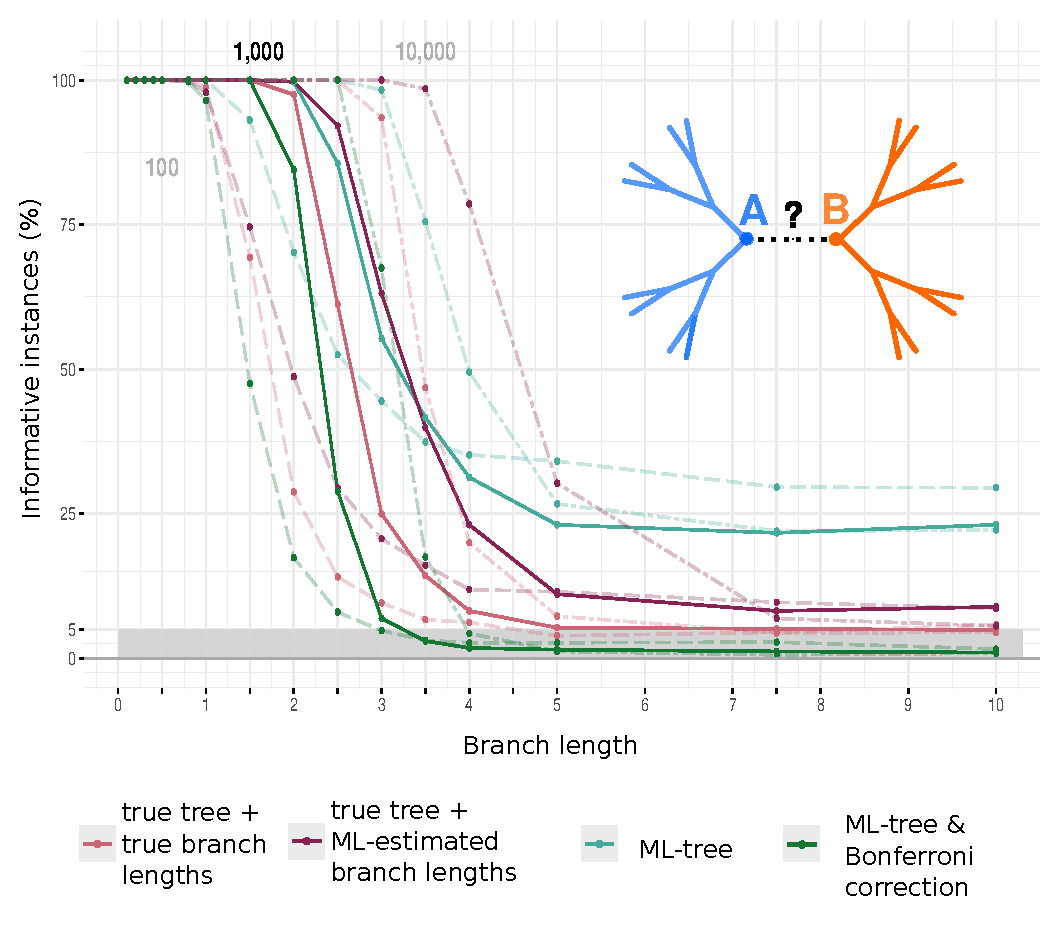
\includegraphics[scale=0.5]{supplementary_figure_effect_short_branches.pdf}
    \vspace{0.25cm}
           \caption{\textbf{Effect of short branches on the test for phylogenetic information.}
           The fraction of phylogenetically informative instances (rejecting the independence of subtrees $\mathbb{T}_A$ and $\mathbb{T}_B$ ) is plotted as a function of the length of branch $AB$ in the true tree in various scenarios: the true tree ({\color{truetree}pink}), the true tree topology with ML-estimated branch lengths ({\color{truetreeML} purple}), and the inferred ML-tree including branch lengths ({\color{MLtree} blue}). The {\color{MLtreeBonferroni} green} curves represent the percentage of informative instances after applying the Bonferroni correction to the light green instances. Dashed, solid and alternating dashed lines represent the results for alignment lengths $100, 1000$ and $10000$, respectively. If many of the branch lengths of the tree are close to zero, then the test with Bonferroni correction becomes conservative and the rejection level falls below $5\%$.}
	\label{suppfig:simulation_shortBranches}
\end{figure}


\textbf{Protocol for Supplementary Fig.\,\ref{suppfig:simulation_shortBranches}:} We closely followed the Protocol for Fig.\,\ref{fig:simulation}b, see Methods \ref{msec:simulations}. The only difference was that the internal and external branch lengths were drawn from the distributions (Fig.\,\ref{suppfig:EvoNAPS_branch_distribution}) of internal and external branch lengths, respectively, as recorded in the EvoNAPS database \citepSupp[\url{http://evonaps.cibiv.univie.ac.at}]{reden2023} with a lower minimum length of $1/n$ (instead of $0.04$), where $n$ is the  alignment length.

\begin{figure}[H]
    \centering
    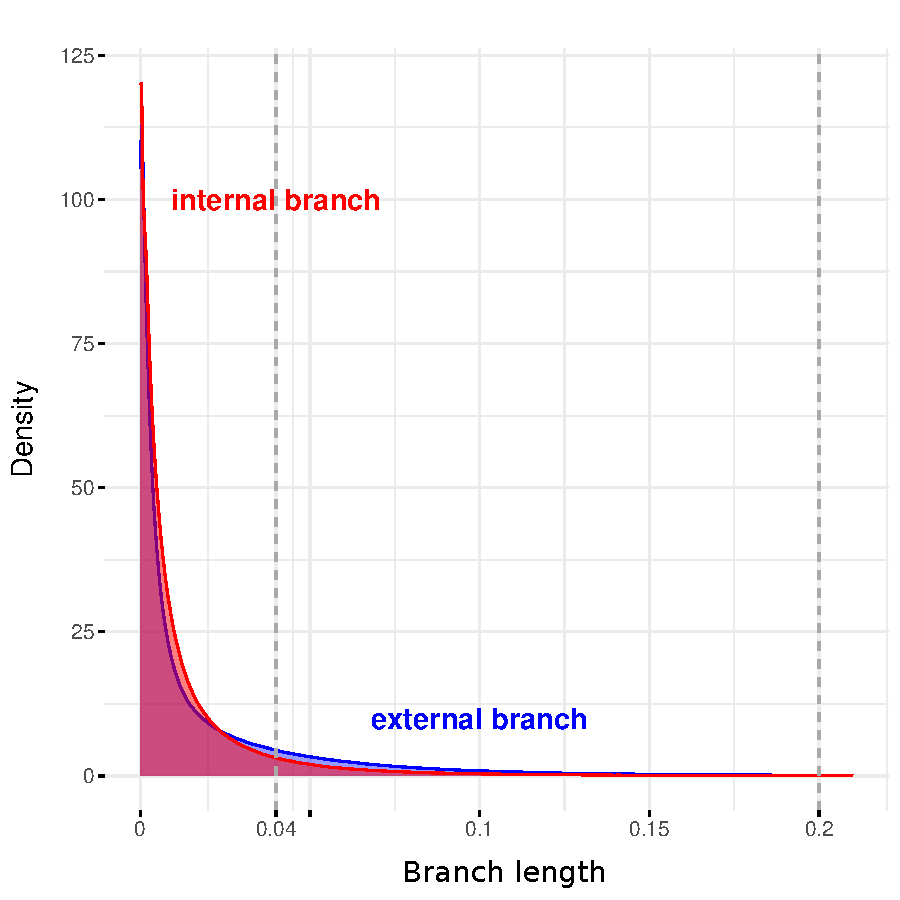
\includegraphics[scale=0.5]{EvoNAPS_branch_length_distribution.pdf}
    \vspace{0.25cm}
    \caption{\textbf{Empirical branch length distribution from EvoNAPS:} The figure shows the distributions of internal and external branch lengths, respectively, as stored in the EvoNAPS database
    %for the sources OrthoMaM, Lanfear and TreeBase
    .}
    \label{suppfig:EvoNAPS_branch_distribution}
\end{figure}

\bigskip

\subsection{Model misspecification simulations}

\begin{figure}[H]
        \centering
        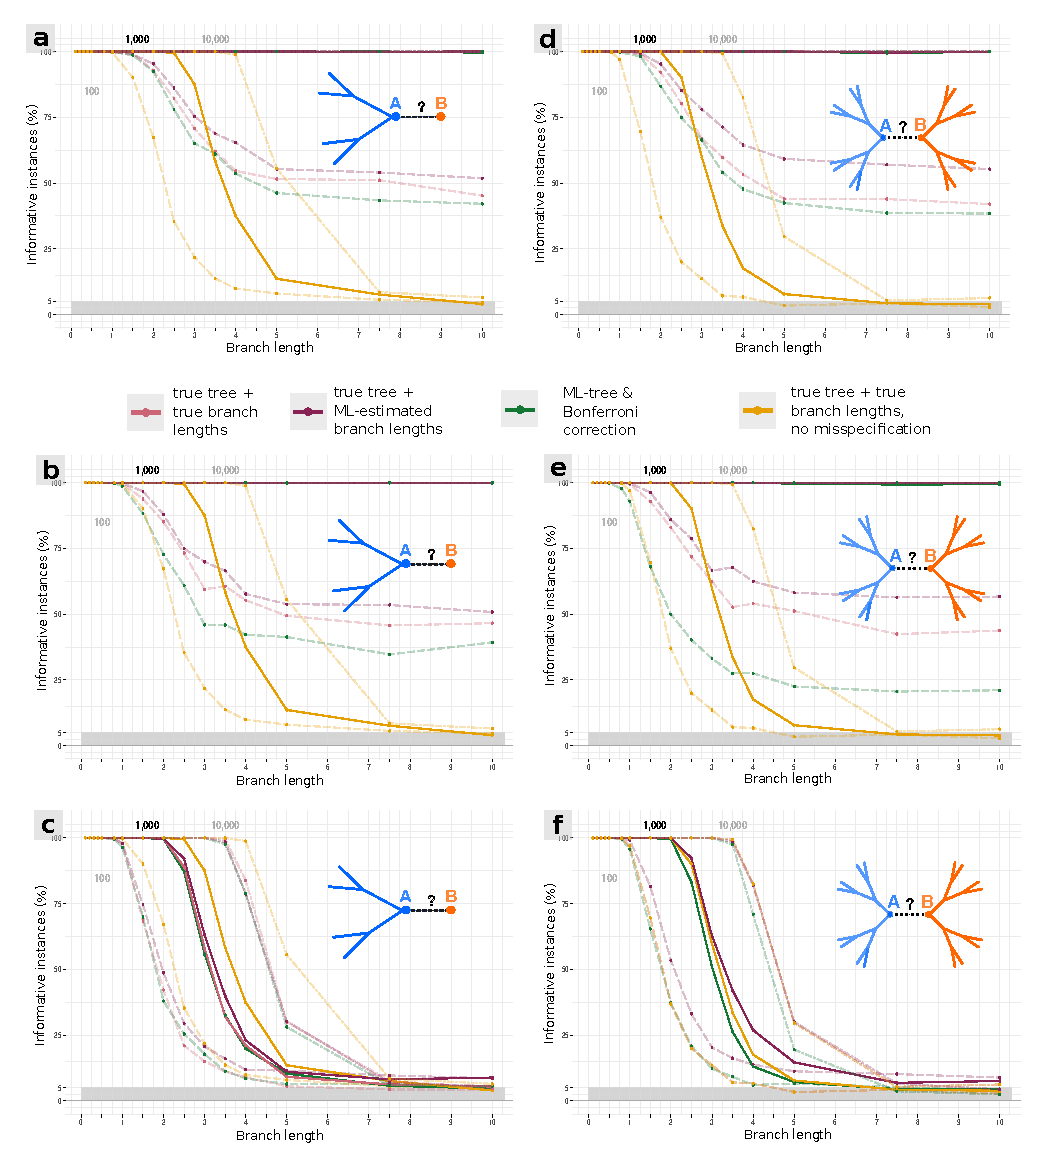
\includegraphics[width=\linewidth]{figure_simulated_data_misspecification.pdf}
             \caption{\textbf{Performance of SatuTe in presence of model misspecification.} The plot shows the fraction of informative instances when testing the branch $AB$ in absence of model misspecification (true-tree, {\color{truetreeNoMisspecification}gold}) and in various scenarios with model misspecification: true-tree ({\color{truetree}pink}), the true-tree topology with ML-estimated branch lengths ({\color{truetreeML} purple}), and the inferred ML-tree including branch lengths with Bonferroni correction ({\color{MLtreeBonferroni} green}). In all cases the alignments were simulated with a GTR model, while reconstruction and testing under model misspecification was performed using the JC \textbf{(a,d)}, K2P \textbf{(b,e)} or F81 \textbf{(c,f)} models. The branches tested were \textbf{(a-c)} the external branch $AB$ of a $5$-taxon tree and \textbf{(d-f)} the central branch $AB$ of a balanced $16$-taxon tree. Dashed, solid and alternating dashed lines represent the results for alignments with $100, 1000$ and $10000$ number of sites, respectively. }
	\label{suppfig:simulation_misspec}
 \end{figure}

\medskip


\noindent\textbf{Protocol for Supplementary Fig.\,\ref{suppfig:simulation_misspec}:} This protocol is similar to the protocol in Methods \ref{msec:simulations}.

\medskip

We consider the same simulation trees as described (for details see M.4. and Table\,\ref{tab:Fig2}). For each parameter combination, we simulated  $1000$ DNA alignments with sequence length ${n = 100, 1000, 10000}$ sites using Seq-Gen \citepMeth[v1.3.4;][]{Rambaut1997} under a GTR model with rates $AC=0.6676$, $AG=3.7807$, $AT=4.2833$, $CG=0.5354$, $CT=0.8718$ and $GT=1.0$ and nucleotide frequencies $\pi_A = 0.125$, $\pi_C = 0.436$, $\pi_G = 0.191$ and $\pi_T =0.245$, as estimated for the best-fit model for the dataset PF06346 stored in the EvoNAPS database \citepSupp[\url{http://evonaps.cibiv.univie.ac.at}]{reden2023}. Each alignment was evaluated using IQ-Tree2 \citepMeth{minh2020} and SatuTe with a significance level of $\alpha = 0.05$ while specifying JC \textbf{(a,d)}, K2P \textbf{(b,e)} and F81 \textbf{(c,f)} as models of substitution instead of GTR. Missing model parameters are estimated from the alignments.


\medskip
The fraction of phylogenetically informative alignments (rejecting the independence of subtrees $\mathbb{T}_A$ and $\mathbb{T}_B$) is plotted as a function of the branch length $AB$ in the simulation tree for four different analyses:

\medskip

\begin{enumerate}
\item  Applying the test for phylogenetic information on the true simulation tree with fixed true branch lengths ({\color{truetreeNoMisspecification}gold}), assuming the GTR model of the simulation for each alignment. (First scenario with good specification)
\item Applying the test for phylogenetic information on the true simulation tree with fixed true branch lengths ({\color{truetree}pink}), assuming the JC \textbf{(a,d)}, K2P \textbf{(b,e)} and F81 \textbf{(c,f)} model for each alignment. (First scenario with model misspecification)
\item Applying the test for phylogenetic information on the true tree topology with ML-estimated branch lengths ({\color{truetreeML} purple}), assuming the JC \textbf{(a,d)}, K2P \textbf{(b,e)} and F81 \textbf{(c,f)} model for each alignment. (Second scenario with model misspecification)
\item Applying the test for phylogenetic information with the  Bonferroni correction $\alpha_{adjust}$ (see Eq.\,\eqref{eq:corrected_significance}) on the inferred ML-tree with estimated branch lengths ({\color{MLtreeBonferroni} green}), assuming the JC \textbf{(a,d)}, K2P \textbf{(b,e)} and F81 \textbf{(c,f)}  model for each alignment. (Fourth scenario with model misspecification) 
\end{enumerate}


%Each datapoint is based on an independent set of $1000$ alignments.

\medskip

Note that, for the GTR model, the second largest eigenvalue has a multiplicity of 1. The JC model \textbf{(a,d)} and the F81 model \textbf{(c,f)} have a unique non-zero eigenvalue with multiplicity $3$. For the K2P model \textbf{(b,e)}, the second largest eigenvalue  has multiplicity $1$ or $2$, depending on the transition/transversion ratio. The details of the test are as described in Methods \ref{msec:test}.

\newpage
\begin{longtable}{|p{.34\textwidth}|p{0.30\textwidth}|p{0.30\textwidth}|}
\hline
   & \textbf{Fig.\,\ref{suppfig:simulation_misspec}a,b,c}&  \textbf{Fig.\,\ref{suppfig:simulation_misspec}d,e,f}\\
      \hline
      \hline
      \multicolumn{3}{|c|}{\textbf{simulation}}\\
      \hline
     \textbf{tree:} & 5-taxon tree & 16-taxon tree\\\hline
     \textbf{branch AB:} & 
        external, see Fig.\,\ref{fig:simulation}a
        & internal, see Fig.\,\ref{fig:simulation}b\\\hline
     \textbf{branches in $\mathbb{T}_A$ \& $\mathbb{T}_B$:} & 
      all 0.2 &
      drawn from EvoNAPS\\
      \hline
     \textbf{\hspace{1em}with length range:} & NA & $0.04$ to $0.2$\\\hline
     \textbf{substitution model:} & GTR model & GTR model \\\hline
      \hline 
      \multicolumn{3}{|c|}{\textbf{evaluation}}\\
      \hline 
     \textbf{substitution model:} &  (a) JC model & (d)JC model \\
     &(b) K2P model &(e) K2P model\\
     & (c) F81 model & (f) F81 model\\
     \hline
     \textbf{Bonferroni correction:} &  
       $\alpha_{adjust} = 0.05/4$ & $\alpha_{adjust} = 0.05/64$\\
   \hline
   \caption{\textbf{SatuTe in simulations with model misspecifications.}}\label{supptab:misspec}
\end{longtable}

Branch lengths of the subtrees $\mathbb{T}_A$ and $\mathbb{T}_B$ in the 16-taxon trees were drawn between $0.04$ and $0.2$ from the distributions of internal and external branch lengths, respectively  (see Supplementary Fig.\,\ref{suppfig:EvoNAPS_branch_distribution}), as stored in the EvoNAPS database \citepMeth[\url{http://evonaps.cibiv.univie.ac.at}]{reden2023}. 

\medskip

Each datapoint in Fig.\,\ref{suppfig:simulation_misspec} has been computed from an independent set of $1000$ alignments.  In the rare cases where the inferred ML-tree did not recover the split induced by branch $AB$ (i.e., the taxa of $\mathbb{T}_A$ did not split from the taxa
of $\mathbb{T}_B$), the ML-tree was discarded. This only occurred for simulated alignments with $n = 100$ and $AB$ branch length $0.1$ or $0.2$ (totalling $4\times1000$ alignments). The maximum number of discarded ML-trees occurred under the F81 model (Fig.\,\ref{suppfig:simulation_misspec}f), where $1.6\%$ ($64$ out of $4\times1000$) of ML-trees where discarded.



%                        AB=0.1, JC:     26+23 = 49/2000 = 2.45 %
%                        AB=0.1, K2P:    20+26 = 46/2000 = 2.3  %
%                        AB=0.1, F81:    28+33 = 61/2000 = 3.05 %
%
%                        AB=0.2, JC:      0+ 2 =  2/2000 = 0.1  %
%                        AB=0.2, K2P:     3+ 0 =  3/2000 = 0.15 %
%                        AB=0.2, F81:     2+ 1 =  3/2000 = 0.15 %

\bigskip

%%% Tab. Bootstrap values %%%
\subsection{Bootstrap support values}
\begin{table}[hb]
    \centering
    \begin{tabular}{|c|r|r|r|r|}
\hline
simulation branch & $AB$ split & Average  & Minimum & Informative\\
length of $AB$& contained   & BS value & BS value & instances (\%) \\
\hline
0.1 &  993 &  93.32 &  14 & 100   \\
0.2 &  999 &  99.19 &  74 & 100  \\
0.3 & 1000 &  99.86 &  87 & 100   \\
0.4 & 1000 &  99.95 &  93 & 100 \\
0.5 & 1000 &  99.99 &  97 & 100   \\
0.8 & 1000 & 100  & 100 &  99.1 \\
1   & 1000 & 100  & 100 &  92.4 \\
1.5 & 1000 & 100  & 100 &  49.7 \\
2   & 1000 & 100  & 100 &  21.6 \\
2.5 & 1000 & 100  & 100 &   9.6 \\
3   & 1000 & 100  & 100 &   5.9 \\
3.5 & 1000 & 100  & 100 &   4.3 \\
4   & 1000 & 100  & 100 &   4.6 \\
5   & 1000 & 100  & 100 &   3.8 \\
7.5 & 1000 & 100  & 100 &   3.5 \\
10  & 1000 & 100  & 100 &   4.3 \\
\hline
    \end{tabular}
    \vspace{0.25cm}
    \caption{
        \textbf{Bootstrap support (BS) values of the simulations for the 16-taxon tree.} For each branch length of $AB$ in the simulation tree as shown in Fig.\,\ref{fig:simulation}b, $1000$ DNA alignments with sequence length of $100$bp were simulated under JC model. For each alignment, we conducted a bootstrap analysis with 100 replicates. The table summarises the number of inferred ML-trees containing a branch that splits the taxa of $\mathbb{T}_A$ and $\mathbb{T}_B$ ($AB$ split contained), along with the average  and minimum bootstrap support values over all $1000$ analyses.  For comparison, we include the fraction of informative instances of Fig.\,\ref{fig:simulation}b for an alignment length of $100$bp in the scenario  ML-tree \& Bonferroni correction (dashed line, {\color{MLtreeBonferroni}green}). 
    }
    \label{supptab:bootstrap}
    \end{table}

\noindent\textbf{Protocol for Table\,\ref{supptab:bootstrap}:} This protocol partially follows the one described for Fig.\,\ref{fig:simulation}b, see Methods \ref{msec:simulations}.

The considered simulation tree is the 16-taxon tree shown in Fig.\,\ref{fig:simulation}b. Our focus is on the internal branch $AB$, which connects the root $A$ of the balanced $8$-taxon subtree $\mathbb{T}_A$ to the root $B$ of thw balanced $8$-taxon subtree $\mathbb{T}_B$. All branch lengths in $\mathbb{T}_A$ and $\mathbb{T_B}$ were drawn between $0.04$ and $0.2$ from the distributions (see Supplementary Fig.\,\ref{suppfig:EvoNAPS_branch_distribution}) of internal and external branch lengths, respectively, as collected in the EvoNAPS database \citepMeth[\url{http://evonaps.cibiv.univie.ac.at}]{reden2023} 
%for the sources OrthoMaM, Lanfear and TreeBase
. As before, the $AB$-branch length was varied among $\{0.1, 0.2, 0.3, 0.4, 0.5, 0.8, 1.0, 1.5, 2.0, 2.5, 3.0, 3.5, 4.0, 5.0, 7.5, 10.0\}$. For each parameter combination, we simulated  $1000$ DNA alignments with sequence length of $100$ sites using Seq-Gen \citepMeth[v1.3.4;][]{Rambaut1997} under the JC model. For each alignment, we conducted a bootstrap analysis with $100$ replicates using IQ-Tree2 \citepMeth{minh2020}. For each of the $1000$ considered ML-tree, we determined if a branch exists that splits the taxa of $\mathbb{T}_A$ and $\mathbb{T}_B$ (i.e., $AB$ split contained). For the ML-trees containing this split, the bootstrap support value of branch $AB$ was computed using $100$ resamplings, allowing us to calculate the average and minimum BS values.


For comparison, we include the fraction of informative instances of Fig.\,\ref{fig:simulation}b for an alignment length of $100$bp in the ML-tree \& Bonferroni correction scenario (dashed line, {\color{MLtreeBonferroni} green}). See  Protocol for Fig.\,\ref{fig:simulation}b (Methods \ref{msec:simulations}).

\medskip
Table\,\ref{supptab:bootstrap} only shows the results for simulated alignments with length $n=100$. For longer alignments ($1000, 10000$) the subtrees were always separated and the BS values were always 100\%, independently of the $AB$ branch length.

\bigskip

%%%%%==============================================================%%%
%%%%%   TREE OF LIFE %%%%%%
    
\newpage
\section{SatuTe and Tree of Life (ToL)}

We apply SatuTe to real data by analysing the Tree of Life (ToL) for ribosomal protein and rRNA alignments.  For this purpose, we are examining the work of \citetSupp{Hug2016}.

\medskip 

Using SatuTe, we can perform a wide range of per-alignment-region analyses considering windows, different proteins or rRNA regions as presented in the main text. Additionally to the insights of the phylogenetic signals for this regions, the resulting z-scores enable us to make comparisons, for instance, between branches or even different topologies. 

\subsection{2D ToL - Ribosomal protein alignment}

\subsubsection{z-score differences between branches}\label{suppsec:2DT_branch_zscore_diffs}

\noindent \textbf{Protocol for  Table \ref{supptab:Eukaryota_Yeast}  and Fig.\,\ref{suppfig:Eukaryota_Yeast}}:
 To compare the phylogenetic signal in protein sequences between branches leading to Eukaryota and baker's yeast (S. cerevisiae), we performed the test according to Methods \ref{msec:hetero} using LG+$\Gamma 4$ model and considering the different proteins. For the comparison, we calculate the difference in per-protein z-scores. The aggregated results are presented in Table \ref{supptab:Eukaryota_Yeast} and Fig.\,\ref{suppfig:Eukaryota_Yeast}.


\begin{table}[ht]
    \centering
    \begin{tabular}{|c|c|c|c|}
\hline
protein & z-score  & z-score & $\Delta$ z-score \\
       & Eukaryota & yeast & (Euk.- Yeast)\\
\hline
L2  & 11.68 & 12.85 & -1.17\\
L3  & 11.62 & 11.38 &  0.24\\
L4  & 11.06 & 12.23 & -1.17\\
L5  & 12.31 & 12.54 & -0.23\\
L6  & 10.34 & 10.49 & -0.15\\
L14 &  9.96 & 10.47 & -0.51\\
L15 &  7.72 &  8.88 & -1.16\\
L16 &  6.35 & 11.30 & -4.95 \\
L18 &  8.23 & 11.82 & -3.59\\
L22 &  8.28 & 11.70 & -3.42\\
L24 &  7.77 &  7.55 &  0.22\\
S3  & 10.85 & 12.81 & -1.96\\
S8  & 10.03 & 10.48 & -0.45\\
S10 &  8.91 &  9.15 & -0.24\\
S17 &  7.92 &  7.23 &  0.69\\
S19 &  8.35 &  8.49 & -0.14\\
\hline

    \end{tabular}
    \vspace{0.25cm}
    \caption{\textbf{Per-protein  z-score comparison between two branches of the 2D ToL.} For each ribosomal protein, the table summarises the the z-score of the branch leading to Eukaryota and yeast in the 2D ToL of Fig.\,\ref{fig:EUK}a, along with their differences. %These differences ($\Delta$ z-score) are represented in Supplementary Fig.\,\ref{suppfig:Eukaryota_Yeast}.
    }
    \label{supptab:Eukaryota_Yeast}
\end{table}

\medskip

\noindent  All z-scores are greater than the critical value $z_\alpha$ or $z_{\alpha_{adjusted}}$ for significance $\alpha = 0.01$. Considering the per-protein z-score difference between Eukaryota and yeast, Supplementary Fig.\,\ref{suppfig:Eukaryota_Yeast} shows that
most of differences in z-score are small or close to zero, with the notable exceptions of L16, L18 and L22, where the Eukaryota branch shows comparatively less phylogenetic signal.

 %The phylogeny-independent saturation index gives z-scores similar in magnitude to those of SatuTe  (Supplementary Figure \ref{fig:indexFigureAA}), although simultaneous variation is much less evident than for the 16S rRNA gene alignment. 



\begin{figure}[ht]
            \centering
            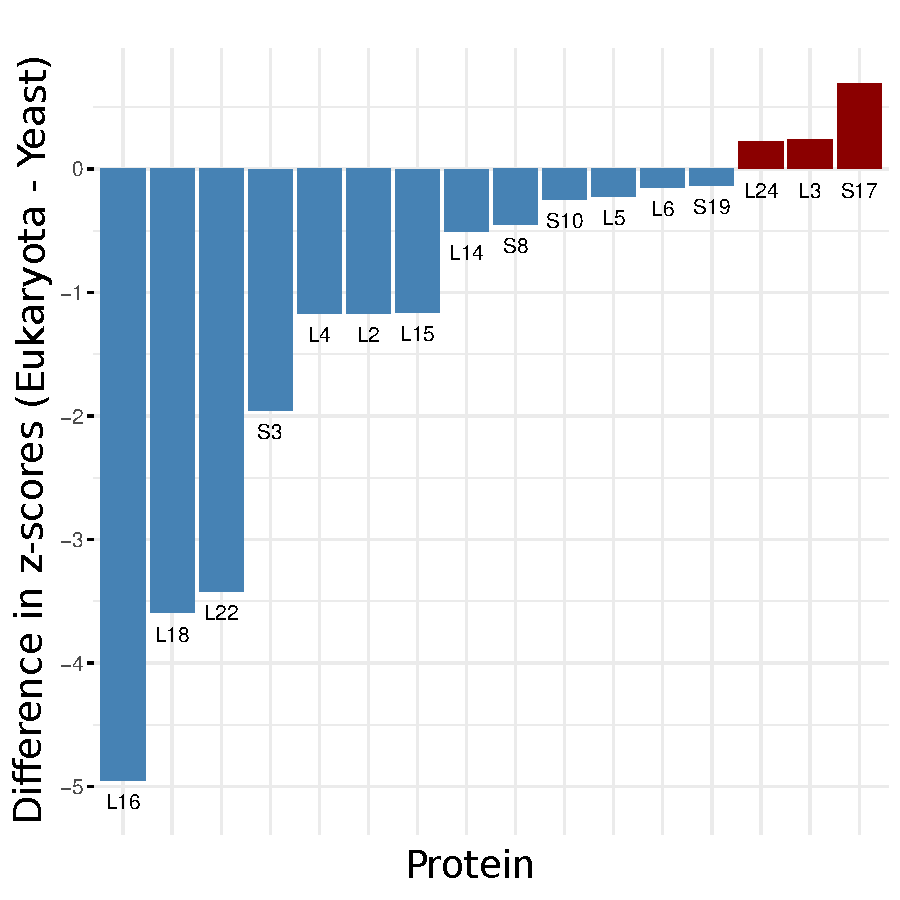
\includegraphics[width=0.65\linewidth]{protein_based_comparison_Yeast_Eukaryota_diff_zscores.pdf}
		     \caption{\textbf{Per-protein z-score comparison between the branches leading to Eukaryota and Yeast.} For each ribosomal protein,  the z-score differences between the branch leading to Eukaryotes and the branch leading to Yeast in the 2D ToL of \mbox{Fig.\,\ref{fig:EUK}a.}  are presented in ascending order.}
		     \label{suppfig:Eukaryota_Yeast}
\end{figure}

\bigskip

\newpage
\subsubsection{z-score differences between topologies}\label{suppsec:2DT_topology_zscore_diffs}

In addition to the branch comparison, z-score differences allow us to determine whether each protein supports the 2D ToL or the 3D ToL.

\medskip

\noindent  \textbf{Protocol for  Table \ref{supptab:protein_2D_3D}:} See the Protocol for Fig.\,\ref{fig:z-score_differences}.

\begin{table}[ht]
    \centering
    \begin{tabular}{|c|r|r|r|r|}
\hline
protein& alignment& z-score & z-score& $\Delta$ z-score\\
&length& 2D ToL & rearranged & (2D-3D)\\
&& & 3D ToL & \\
\hline
L2&317&11.68&11.65& 0.03\\
L3&228&11.62&11.07& 0.55\\
L4&245&11.06&11.02& 0.04\\
L5&164&12.31&12.21& 0.10\\
L6&220&10.34&10.27& 0.07\\
L14&125&9.96&9.01& 0.95\\
L15&122&7.72&8.75& -1.03\\
L16&153&6.35&6.30& 0.05\\
L18&141&8.23&8.11& 0.12\\
L22&174&8.28&8.69& -0.41\\
L24&81&7.77&7.68& 0.09\\
S3&216&10.85&10.51& 0.34\\
S8&141&10.03&9.77& 0.26\\
S10&104&8.91&9.04& -0.13\\
S17&74&7.92&7.37& 0.55\\
S19&91&8.35&8.01& 0.34\\
\hline
    \end{tabular}
    \vspace{0.25cm}
    \caption{\textbf{Per-protein z-score comparison to a rearranged topology:} For each ribosomal protein, the table summarises the z-scores of the branch leading to Eukaryota in the 2D ToL of Fig.\,\ref{fig:EUK}a and the 3D-rearranged tree of Fig.\,\ref{fig:z-score_differences}a, along with their differences. %The sorted difference in z-score between the two trees for the branch leading to Eukaryota ($\Delta$z-score) is represented in Fig.\,\ref{suppfig:2D_z-score_differences}.
    }
    \label{supptab:protein_2D_3D}
    \end{table}

%\medskip
%
%The z-score difference of Fig.\,\ref{fig:z-score_differences} sorts all ribosomal proteins from those favouring the rearranged 3D ToL to those favouring the 2D ToL. Following this ordering, the alignment composed by ribosomal proteins L15, L22, S10 and L2 is the smallest alignment with no sequences composed uniquely by gaps. For this initial alignment, branch lengths were ML-estimated for both the 2D ToL and the rearranged 3D ToL, giving the difference in log-likelihood ${L_{2D}-L_{3D}}$, see  Supplementary Table \ref{supptab:likelihood_2D_3D}.
%
%\medskip 
%
%\noindent  \textbf{Protocol for Table \ref{supptab:likelihood_2D_3D}}: 
% For the 2D ToL in Fig.\,\ref{fig:EUK}a and  the rearranged 3D ToL in Fig.\,\ref{fig:z-score_differences}a, we determine the log-likelihood for different alignments. {\color{red}To do this, branch length are inferred using an LG+G4 model for each alignment.} Starting with the alignment of L15, L22, S10 and L2, we progressively extended the considered alignment by adding the next protein with the smallest z-score difference, which is L4. Then, we compute the  log-likelihood  differences ${L_{2D}-L_{3D}}$. This process is repeated by adding ribosomal proteins L16 and L15.
%
%
%\begin{table}[ht]
%    \centering
%\begin{tabular}{ | m{3cm} | m{2cm}| }  
%  \hline
%  Proteins included & $L_{2D}-L_{3D}$\\ 
%  \hline
%  L15, L22, S10, L2 & -32.83 \\ 
%  \hline
%  + L4 & -7.10 \\ 
%   \hline
%  + L16 & 11.84 \\ 
%   \hline
%  + L15 & 17.12 \\ 
%  \hline
%\end{tabular}
%\caption{Difference in log-likelihood between the 2D ToL and the rearranged 3D ToL for different subalignments. We progressively extend the original alignment of proteins L15, L22, S10, L2  by adding the next protein with the minimum  z-score difference  (Fig.\,\ref{fig:z-score_differences}b). }
%\label{supptab:likelihood_2D_3D}
%\end{table}

\medskip
\newpage
\subsection{3D ToL - 16S rRNA alignment}\label{suppsec:rRNA_based_3DT}

\subsubsection*{z-score differences between topologies}\label{suppsec:3DT_topology_zscore_diffs}

For comparison,  we  determine  the z-score differences of different rRNA regions for the 2D or the 3D ToL.

\medskip

\noindent  \textbf{Protocol for  Table \ref{supptab:rRNA_2D_3D}:} We divided the 16S rRNA gene alignment into nine distinct rRNA-regions, as detailed in Table \ref{supptab:rRNA_2D_3D}. See the Protocol for Fig.\,\ref{fig:z-score_differences}.

\medskip

\begin{table}[ht]
    \centering
    \begin{tabular}{|c|c|c|c|c|}
\hline
region&site& z-score & z-score& $\Delta$ z-score\\
&range&3D ToL & rearranged & (2D-3D)\\
&& & 2D ToL & \\
\hline
R1&0-114&4.57&5.08&0.51\\
R2&115-431&6.13&5.94&-0.19\\
R3&432-621&3.63&3.45&-0.17\\
R4&622-1066&6.81&6.83&0.03\\
R5&1067-1221&8.99&8.93&-0.06\\
R6&1222-1394&8.55&8.31&-0.23\\
R7&1395-1565&8.93&8.35&-0.59\\
R8&1566-1765&12.44&12.33&-0.12\\
R9&1766-1946&9.33&9.65&0.33\\
\hline
    \end{tabular}
    \vspace{0.25cm}
    \caption{\textbf{Per-region z-score comparison to a rearranged topology} For each rRNA region, the table summarises the z-scores of the branch leading to Eukaryota in the ML-reconstructed 3D ToL (Fig.\,\ref{fig:EUK}d) and the rearranged 2D ToL (Fig.\,\ref{fig:z-score_differences}c), along with their differences.}
    \label{supptab:rRNA_2D_3D}
    \end{table}

%\noindent \textbf{Results:} Paradoxically, the 16S rRNA belongs to the small ribosomal subunit, while the 16S rRNA gene favours the 3D ToL of life for $6$ out of $9$ regions when an analogous 2D-rearranged tree is constructed (Fig.\,\ref{suppfig:rRNA_2D_3D}). This suggests that explaining the disagreement between the 16S rRNA and its surrounding proteins (see Section \ref{suppsec:2DT_topology_zscore_diffs}) could be a useful hint to find a reliable reconstruction of the Tree of Life.

\end{appendices}
\begin{appendices}
\setcounter{section}{2} 

%%%%%%%%==================================================%%%%%
%%%%% MATH PART %%%%%%%
\section{Theoretical foundation of SatuTe}\label{suppsec:maths}
\subsection{Basic properties of the coherence coefficient}
\label{sec:apx}

As inferred from Eq.\,\eqref{eq:branchlikelihod_new}, for pattern $\partial$ the coherence coefficient corresponding to eigenvalue $\lambda_i$ is defined as
\begin{equation} \label{eq:coherence_again}
    C^\partial_i := \langle \frac{\va}{\Prob(\pred)},\bm{h_i}\rangle \langle \frac{\vb}{\Prob(\pblue)}, \bm{h_i}\rangle.
\end{equation}

Let us restate the spectral decomposition of Eq.\,\eqref{eq:spectral_decomposition}. Due to reversibility, the transition matrix $\bm{P}(t) = e^{Qt}$ decomposes as 

\begin{align} \label{eq:spectral_decompositionAppendix}
   \bm{P}(t) = \bm{1}\bm{\pi}^T + \sum_{i=1}^3\bm{v_i} \bm{h_i}^T e^{\lambda_it},
\end{align}
 
where  ${\lambda_0 = 0 > \lambda_1 \geq \lambda_2 \geq \lambda_3}$  are the eigenvalues of the rate matrix and $\bm{h_i}, \bm{v_i}$  are the corresponding left and right eigenvectors. 
Note that the right eigenvalues form an orthonormal basis with respect to $\bm{\pi}$-inner product $\langle \bm{v},\bm{w}\rangle_{\bm{\pi}}= \bm{v}^T\cdot\diag(\bm{\pi})\cdot\bm{w}$ and $\bm{h}_k=\diag(\bm{\pi})\bm{v}_k$ \citepMain{levin2017markov}.


\medskip


To simplify the computation of the expected value of the coherence coefficient, in Prop. \ref{prop:totalSumLikelihood} we consider each scalar product of Eq.\,\eqref{eq:coherence_again} independently.

\begin{prop}\label{prop:totalSumLikelihood} Assuming stationarity, for each pattern $\pred$ observed at the tips of subtree $\mathbb{T}_A$, consider the likelihood vector $\va$ and  the probability ${\Prob(\pred) = \langle \bm{\pi},  \va \rangle }$. The following holds.

\smallskip


\begin{enumerate}[label=\alph*)]
\item If $\bm{1}$ denotes the column vector of $1$'s, then
\begin{equation*} \label{eq:expected1}
\mathbb{E}\Big[\frac{\va}{\Prob(\pred)}\Big] = \bm{1}.
 \end{equation*}
\item If vector $\bm{h_i}$ is orthogonal to $\bm{1}$, then it holds that
 \begin{equation*}\label{eq:expectedscalar0}
 \mathbb{E}\Big[\langle \frac{\va}{\Prob(\pred)}, \bm{h_i}\rangle\Big] = 0.
 \end{equation*}
 \end{enumerate}
\end{prop}
\begin{proof} \hfill


\begin{enumerate}[label=\alph*)]
\item It  is enough to show that 
 \begin{equation} \label{eq:sum1}
      \sum _\pred \va = \bm{1}.
 \end{equation}
Consider one nucleotide $i$. Focusing on the $i$th entry of $\va$, we see that \[\sum_\pred \Prob(\pred  \mid  \text{$i$ at node $A$}) = 1\]
because we are summing over all possible outcomes $\pred$, as desired.
\item We just need to use linearity and item $a)$. Indeed,
\begin{equation}
\mathbb{E}\Big[\langle \frac{\va}{\Prob(\pred)}, \bm{h_i}\rangle\Big] =\langle  \mathbb{E}\Big[\frac{\va}{\Prob(\pred)}\Big], \bm{h_i}\rangle = \langle  \bm{1}, \bm{h_i}\rangle = 0,
\end{equation} 
where in last equality we used the fact that $\bm{h_i}$ and $\bm{1}$ are orthogonal, as it is the case in the spectral decomposition of Eq.\,\eqref{eq:spectral_decompositionAppendix}.
%, as stated in Equation \ref{eq:decomposition}.
\end{enumerate}
\end{proof}

Recall that Eq.\,\eqref{eq:centraleq} implies that, when the length of branch $AB$ grows, the subpatterns $\pred$ and $\pblue$ become independent. Using Prop. \ref{prop:totalSumLikelihood}, we can easily compute the expected value $\mathbb{E}[C^\partial_i]$ under the assumption of subtree independence as follows. 

\begin{prop} \label{prop:CoherenceToZero} In a phylogenetic tree $\mathbb{T}$, consider a branch $AB$ with length $t \to \infty$. Assuming stationarity and reversibility, for any $i \in \{1,2,3\}$ it holds that 
    \[ \mathbb{E}[C^\partial_i] = 0.\]
\end{prop}
\begin{proof}
Since subpatterns $\pred$ and $\pblue$ are sampled independently, also $\langle \va/\Prob(\pred),\bm{h_i}\rangle$ and $\langle \vb/\Prob(\pblue), \bm{h_i} \rangle$ are independent. The expectation is multiplicative under independence, and thus we have
 \begin{align}
    \mathbb{E}[C^\partial_i] &= \mathbb{E}\Big[  \langle \frac{\va}{\Prob(\pred)},\bm{h_i}\rangle \langle \frac{\vb}{\Prob(\pblue)}, \bm{h_i} \rangle \Big] =  \\
    &=  \mathbb{E}\Big[  \langle \frac{\va}{\Prob(\pred)},\bm{h_i}\rangle \Big] \mathbb{E}\Big[ \langle \frac{\vb}{\Prob(\pblue)}, \bm{h_i} \rangle \Big] = 0,
\end{align}
where we used Prop. \ref{prop:totalSumLikelihood}b.

\end{proof}

As described in Methods \ref{msec:estimates}, for any $i,j\in \{ 1,2,3\}$ we define the covariance
\begin{equation}\sigma^2_{A,i,j}:=\mathbb{E}\Big[\langle \frac{\va}{\Prob(\pred)},\bm{h_i}\rangle  \langle \frac{\va}{\Prob(\pred)},\bm{h_j}\rangle \Big] 
%= \cov [\langle \frac{\va}{\Prob(\pred)},\bm{h_i}\rangle, \langle \frac{\va}{\Prob(\pred)},\bm{h_j}\rangle]
.\end{equation}

This is indeed the covariance between the two scalar products due to Prop. \ref{prop:totalSumLikelihood}b. As claimed in Methods \ref{msec:estimates}, in the following proposition we prove that $\sigma^2_{A,i,j}$ greatly simplifies if node $A$ is external. 

\begin{prop} \label{prop:memorySequence}
    Assuming stationarity and reversibility, if node $A$ is external (or equivalently, if subtree $\mathbb{T}_A$ is composed by a single sequence), then \[
    \sigma^2_{A,i,j} =  \begin{cases}
    1,  & \text{if $i=j$}.\\
    0,&  \text{if $i\neq j$}.
    \end{cases}
    \]
\end{prop}
\begin{proof}
   In the eigendecomposition of Eq.\,\eqref{eq:spectral_decompositionAppendix}, we know that $\diag(\bm{\pi}) \bm{v_i} = \bm{h_i}$, while $\langle \bm{v_i} ,\bm{h_j} \rangle = 1$ and $\langle \bm{v_i} ,\bm{h_j} \rangle = 0$ if $i \neq j$. The patterns of a single sequence are the possible letters $x$ it is composed of.  Moreover, due to stationarity, we know that pattern $\pred = x$ satisfies $\Prob(\pred) = \pi_x$, where $x$ is a nucleotide. Note also that, if $\pred = x$,  then $\bm{L}(\pred)$ is the vector of $0$'s, except $1$ at the $x$th entry. All in all, we have
\begin{equation}
\sigma^2_{A,i,i} = \sum_x \Prob(x) (\frac{1}{\pi_x} h_i^x )^2 = \sum_x \pi_x (\frac{1}{\pi_x} h_i^x )^2 = \sum_x v_i^x h_i^x = \langle \bm{h_i}, \bm{v_i} \rangle= 1.
\end{equation}
Similarly, if $i \neq j$ we have 
\begin{equation}
  \sigma^2_{A,i,j}   = \sum_x \Prob(x) (\frac{1}{\pi_x} h_i^x )(\frac{1}{\pi_x} h_j^x ) = \sum_x \pi_x (\frac{1}{\pi_x} h_i^x )(\frac{1}{\pi_x} h_j^x ) = \langle \bm{h_i}, \bm{v_j} \rangle = 0.
\end{equation}
\end{proof}


\subsection{Testing for Saturation for Any Multiplicity of \texorpdfstring{$\lambda_1$}{l1}}
\label{sec:multiplicityGreaterThan1}

Any linear combination of the coherence coefficients them can be used to test for saturation. However, we want the most powerful test among the candidates. As we prove in Appendix \ref{subsec:approximation}, optimal power is achieved asymptotically by the test that uses the coherence coefficient introduced in Eq.\,\eqref{eq:estimator_explicit}, namely
\begin{equation}\label{eq:dominant_coherence}
\hat{C}_1:= \sum_{k \in \{ 1, \cdots , D \}}\hat{C}_{1, k},
\end{equation} 
where eigenvalue $\lambda_1$ has multiplicity $D$ and $\lambda_1 = \cdots = \lambda_D$. Under the null hypothesis of subtree independence, the expectation and variance of $\hat{C}_1$ can be computed as described in the following proposition.

\medskip
 
\begin{prop} \label{prop:variance_coherence_D}  In a phylogenetic tree $\mathbb{T}$ consider a branch $AB$ with length $t^*$ and assume stationarity and reversibility.  If $t^* \to \infty$, then the coherence coefficient $\hat{C}_1$ satisfies
\begin{align}
 \mathbb{E}[\hat{C}_1] &= 0,\\
 \mathrm{Var}[\hat{C}_1] &= \frac{1}{n}\sum_{i, j \in \{1,\cdots, D\}} 
   \sigma^2_{A,i,j}   \sigma^2_{B,i,j}.
\end{align}
In particular, if node $A$ is external, then 
\begin{equation} \label{eq:externalMultiple}
 \mathrm{Var}[\hat{C}_1]= \frac{1}{n}\sum_{i \in \{1,\cdots, D\}} 
      \sigma^2_{B, i, i},
\end{equation}
and if both nodes $A$ and $B$ are external, then 
\begin{equation}
 \mathrm{Var}[\hat{C}_1] = \frac{D}{n}.
 \end{equation}
\end{prop}
\begin{proof} Since the expectation of a sum is the sum of expectations, $\mathbb{E}[C_{1,i}^\partial] = 0$ (Prop. \ref{prop:CoherenceToZero}) implies that  $\mathbb{E}[\hat{C}_1] = 0$. 
 
 \medskip
 
 Regarding the variance, we can sum up the variance of each independent site, giving $\mathrm{Var}[\hat{C}_1] = 1/n  \mathrm{Var}[\sum_{i \in \{1,\cdots,D\}}C^\partial_{1,i}] $. Since $\mathbb{E}[C^\partial_{1,i}] = 0$ (Prop. \ref{prop:CoherenceToZero}), we have 
 \begin{equation} \label{eq:VarianceExpected}
     \mathrm{Var}[\sum_{i \in \{1,\cdots, D\}}C^\partial_{1,i}] =\mathbb{E}[(\sum_{i \in \{1,\cdots, D\}}C^\partial_{1,i})^2 ].
 \end{equation}
 After expanding the squared sum $(\sum_{i \in \{1,\cdots, D\}}C^\partial_{1,i})^2$, since the expectation is multiplicative under independence, a summand 
 $C^\partial_{1,i} C^\partial_{1,j}$ satisfies
  \begin{align}
 &\mathbb{E}[C^\partial_{1,i} C^\partial_{1,j}] = \\
 =& \mathbb{E}\Big[\langle \frac{\va}{\Prob(\pred)},\bm{h_i}\rangle \langle \frac{\vb}{\Prob(\pblue)}, \bm{h_i} \rangle \langle \frac{\va}{\Prob(\pred)},\bm{h_j}\rangle \langle \frac{\vb}{\Prob(\pblue)}, \bm{h_j} \rangle\Big]= \nonumber\\
  =& \mathbb{E}\Big[\langle \frac{\va}{\Prob(\pred)},\bm{h_i}\rangle \langle \frac{\va}{\Prob(\pred)},\bm{h_j}\rangle \Big]  \mathbb{E}\Big[\langle \frac{\vb}{\Prob(\pblue)}, \bm{h_i} \rangle \langle \frac{\vb}{\Prob(\pblue)}, \bm{h_j} \rangle\Big]= \nonumber\\
  =& \sigma^2_{A,i,j}   \sigma^2_{B,i,j}.\nonumber
 \end{align}
 Summing for all $i,j \in \{1,\cdots, D\}$ we get the desired equality.  The particular case when nodes $A$ and/or $B$ are external follows from Prop. \ref{prop:memorySequence}.
 
\end{proof}


Prop. \ref{prop:variance_coherence_D} leads to a one-sided $z$-test based on the coherence coefficient $\hat{C}_1$. The null hypothesis of independence is rejected with significance $\alpha$ if 
\begin{equation} \label{eq:threshold_D}
     \hat{C}_1 >  z_\alpha \sqrt{
     {\mathrm{\widehat{Var}}}[\hat{C}_1]
     } = z_\alpha \frac{\sqrt{\sum_{i, j \in \{1,\cdots, D\}} 
   \hat{\sigma}^2_{A,i,j}   \hat{\sigma}^2_{B,i,j}.
}}{\sqrt{n}},
\end{equation} where $z_\alpha$ satisfies $\Prob(Z > z_\alpha) = \alpha$, while $\hat{\sigma}^2_{A,i,j}$ is the sample estimate of $\sigma^2_{A,i,j}$ introduced in Eq.\,\eqref{variance_estimate}. If node $A$ is external, then Eq. \ref{eq:threshold_D} is simplified due to Prop. \ref{prop:memorySequence} as 
\begin{equation} \label{eq:threshold_D_external}
     \hat{C}_1 > z_\alpha \frac{\sqrt{\sum_{i\in \{1,\cdots, D\}}  \hat{\sigma}^2_{B,i,i}
}}{\sqrt{n}}.
\end{equation}
\bigskip

\subsection{The Asymptotic Equivalence between the MLE and the Dominant Coherence
}
\label{sec:asym_phylo_tree}

There is a close relationship between the coherence coefficient and the log-likelihood of a branch. To describe this relationship, consider branch $AB$ of tree $\mathbb{T}$. Given an alignment where pattern $\partial$ is observed $n_\partial$ times, the log-likelihood $f(t)$ of branch $AB$ having length $t$ is
\begin{equation}\label{eq:definitionloglike}
f(t) = 
\sum_\partial n_\partial \log{(\Prob(\partial \mid t))}.
\end{equation}
If we define the log-likelihood of independence as 
 \begin{equation} \label{eq:DIFLoglikelihood}
 {f_\infty := \sum_\partial n_\partial \Big(\log\Prob(\pred)+  \log\Prob(\pblue)\Big)}, 
 \end{equation}
 then Eq.\,\eqref{eq:definitionloglike} can be rewritten as 
\begin{equation}\label{eq:definitionloglike2}
f(t) -f_\infty= 
\sum_\partial n_\partial \log{(\frac{\Prob(\partial \mid t)}{\Prob(\pred)\Prob(\pblue)})}.
\end{equation}
    Using Eq.\,\eqref{eq:centraleq}, last equation becomes
 \begin{align} 
     \label{eq:efficient_likelihood_2}
     f(t)-f_\infty &=  \sum_{\partial} n_\partial \log \Big( 1+  \sum_{i \in \{1,2,3\}} e^{\lambda_it}  C_i^\partial\Big).
 \end{align} 
 
In Prop. \ref{prop:limit_likelihood_tree},  we formalise the relationship between the coherence coefficient and the log-likelihood $f(t)$. 
 
  \begin{prop} \label{prop:limit_likelihood_tree}
Assuming stationarity and reversibility, if rate matrix $Q$ has eigenvalues $0 > \lambda_1 \geq \lambda_2 \geq \lambda_3$ and $\lambda_1$ has multiplicity $D$, then define the coherence coefficient \[\hat{C}_1 := \sum_{i \in \{1,\cdots, D\}} \hat{C}_{1,i}.\]
If $\hat{C}_1 \neq 0,$ then \[f(t) - f_\infty \sim \hat{C}_1 n e^{\lambda_1 t}.\]
\end{prop}
\begin{proof} \hfill
 \begin{sloppypar}
 In Equation \ref{eq:definitionloglike2} it is clear that $f(t) - f_\infty$ tends to zero as $t \to \infty$, since $\log(1) = 0$. Now, using L'H\^{o}pital's rule, it is enough to show that the derivative $f'(t)$ satisfies ${f'(t) \sim 
     \hat{C}_1 n \lambda_1  e^{\lambda_1 t}}$. In the expression
 \end{sloppypar}
 \begin{equation*}
     [\log \Big(1 +  \sum_{i \in \{ 1,2,3\}} e^{\lambda_i t} C_i^\partial \Big)]' = \frac{  \sum_{i \in \{ 1,2,3\}} \lambda_i e^{\lambda_it} C_i^\partial }{1 + \sum_{i \in \{ 1,2,3\}} e^{\lambda_it} C_i^\partial},
 \end{equation*}
 the denominator is asymptotically equivalent to $1$. On the other hand, if ${\sum_{i \in \{1,\cdots, D\}}C_i^\partial \neq 0,}$ then the numerator is equivalent to ${\lambda_1e^{\lambda_1t}\sum_{i \in \{1,\cdots, D\}}C_i^\partial}$, and $o(e^{\lambda_1t})$ otherwise. Due to the assumption $\hat{C}_1 \neq 0$, we can sum up the equivalencies, giving
\begin{equation}
     f'(t) \sim \sum_{\partial} n_\partial \Big(
     \lambda_1 e^{\lambda_1t}
     \sum_{i \in \{1,\cdots, D\}}
     C_{1,i}^\partial 
     \Big) = 
     n \lambda_1  e^{\lambda_1 t} \sum_{i \in \{1,\cdots, D\}} 
     \hat{C}_{1,i}= n \lambda_1  e^{\lambda_1 t} \hat{C}_1,
\end{equation}
as desired.

\end{proof}

\iffalse
Notably, Prop. \ref{prop:limit_likelihood_tree} implies that whether $f(t)$ increases or decreases for large $t$ uniquely depends on the sign of $\hat{\delta}$, as stated in the following corollary. 

\begin{cor} \label{prop:decission_tree}
\begin{sloppypar}
Given an alignment and assuming a stationary and reversible process on a tree, the log-likelihood $f(t)$ of branch $AB$ having length $t$ satisfies the following.

\end{sloppypar}
\begin{itemize}
    \item[a)] If $\hat{\delta}$ is positive, then $f(t)$ has local minimum $f_\infty$ when $t \to \infty$.
    \item[b)] If $\hat{\delta}$ is negative, then $f(t)$ has local maximum $f_\infty$ when $t \to \infty$.
\end{itemize}
\end{cor}
Corollary \ref{prop:decission_tree} is an additional motivation (apart from the approximation of the likelihood-ratio test in Subappendix \ref{subsec:approximation}) to perform a one-sided test for saturation in Equations \ref{eq:threshold} and \ref{eq:threshold_D}. Indeed, it would be contradictory to reject saturation because  $\hat{\delta} \ll 0$, while the MLE could be $\hat{t} = \infty$ due to Cor. \ref{prop:decission_tree}b. 

\fi

%Leaving aside our test for saturation, we recommend using Corollary \ref{prop:decission_tree} to predict the possible numerical divergence of the Newton method. If the log-likelihood $f(t)$ has a unique maximum for $t \in [0, \infty]$, Corollary \ref{prop:decission_tree} characterizes the convergence of the Newton method  in the search for the absolute maximum of $f(t)$. %as explained in Appendix \ref{sec:multiple_maxima}. For practitioners, 
 %However, in general Corollary \ref{prop:decission_tree} cannot be used to guarantee that an MLE $\hat{t} < \infty$ is indeed the absolute maximum point, since the log-likelihood $f(t)$ can have multiple maxima.
 
 \subsection{Optimal power of the test for saturation}
\label{subsec:approximation}
We know that the likelihood-ratio test is the most powerful $\alpha$-level test, as proved by \citeSupp{Neyman1933}. 
%In Appendix  \ref{sec:asym_phylo_tree}, we have described the the log-likelihood $f(t)$ of branch $AB$ having length $t$, which has limit $f_\infty$ as $t \to \infty$ (Equations \ref{eq:definitionloglike}, \ref{eq:DIFLoglikelihood}, and \ref{eq:definitionloglike2}). 
Given the log-likelihood $f(t)$ of branch $AB$ having length $t$, if the MLE is $\hat{t} < \infty$, the likelihood-ratio test compares the null hypothesis $t^* \to \infty$ versus the alternative hypothesis $t^* = \hat{t}$  using statistic $f(\hat{t})-f_\infty$, or more explicitly
\begin{equation}
    \text{"Reject $t^* \to \infty$ if $f(\hat{t})-f_\infty > c$",}
\end{equation}
 where $c \in \mathbb{R}_{>0}$ is chosen so that $\Prob(f(\hat{t})-f_\infty > c  \mid  t^* \to \infty) = \alpha$.


\medskip
Assuming that $\hat{t}$ is large enough,
%from the singularity of $f(t)$, 
we can use the approximation ${f(\hat{t}) \approx  f_\infty + \hat{C}_1 n e^{\lambda_1 \hat{t}}}$ of Prop. \ref{prop:limit_likelihood_tree}. This gives the test 
\begin{equation}
    \text{"Reject $t^* \to \infty$ if $ \hat{C}_1  > e^{-\lambda_1 \hat{t}}c/n$",}
\end{equation}
 where $c \in \mathbb{R}_{>0}$ is chosen so that $\Prob( \hat{C}_1 > e^{-\lambda_1 \hat{t}}c/n \mid  t^* \to \infty) = \alpha$. Setting $c' := e^{-\lambda_1 \hat{t}}c/n$, it is clear that the one-sided test for saturation using the coherence coefficient $\hat{C}_1$ achieves optimal power for long branches. 


\bibliographystyleSupp{apalike}
\bibliographySupp{biblio.bib}


\end{appendices}



\end{document}